\chapter{Efficient Conflict Detection of Change-based Models}
\label{ch:conflict_detection}
  
In Chapter \ref{ch:model_differencing}, this work have demonstrated that  change-based model persistence can be exploited to speed up model differencing. In this Chapter, this work extends the proposed approach in Chapter \ref{ch:model_differencing} also by leveraging change-based model persistence to improve the performance of conflict detection in model versioning. The proposed approach can substantially reduce conflict detection time (up to 90\% in some experiments) compared to state-based model differencing. 

\section{Introduction}
\label{sec:introduction_7}
State- and change-based model conflict detection have been discussed briefly in Sections \ref{sec:emfcompare_conflict_detection} and \ref{sec:emfstore_conflict_detection}. The state-based approach, represented by EMF Compare \cite{emfcompare2018developer}, does come with drawbacks. First, it cannot detect conflicts as accurate as change-based approach can as their changes are derived -- not the real historical changes. Second, EMF Compare uses 3-way model comparison \cite{emfcompare2018developer} thus hypothetically its conflict detection should perform relatively slower than the change-based approach, since it has to perform state-based model differencing twice to derive changes events: changes events between left and original versions, and change events between right and original versions. 

Change-based model conflict detection \cite{koegel2010operation}, represented by EMF Store \cite{emfstore2019what}, also has drawbacks. EMF Store purely works on comparing change events and detects conflicts based on predefined rules; it does not consider the eventual states of two versions that are being compared. Thus, two change events that modifies a same feature are considered in conflict even though both change events produce the same eventual states. This condition can lead EMF Store to oversensitive conflict detection. In terms of performance, as has been presented in Chapter \ref{ch:model_differencing}, the change-based approach is faster than its state-based counterparts in model differencing. Thus, it is expected that it can also performs better that the state-based approach in detecting conflicts.
 
In this Chapter, this work proposes a change-based model conflict detection that also considers the eventual states of modified elements. Thus, the performance and accuracy of model conflict detection can be improved, compared to state-based approach, without being oversensitive.
 
\section{Epsilon Change-based Model Conflict Detection}
\label{epsilon_change_based_model_conflict_detection}
The model conflict detection proposed in this study basically performs similar procedure to the phases of change-based model differencing discussed in Chapter \ref{sec:change_based_approach_for_comparing_models} except that (1) it only executes event loading and element tree construction phases and replaces diff computation phase with conflict computation phase, and (2) during element tree construction, it maps change events to the elements, features, and values that they modify. The change event mapping and conflict computation are discussed in the following Sections.

\subsection{Change Event Mapping}
\label{sec:change_event_mapping}
Using the information contained in change-based model persistence in Listings \ref{lst:cbp_right} and \ref{lst:cbp_left}, we can construct an element tree as depicted in Figure \ref{fig:right_element_tree_diagram} using the construction method presented in Section \ref{sec:tree_construction}. During the the construction, change events in Listings \ref{lst:cbp_right} and \ref{lst:cbp_left} are mapped to the affected elements, features, and values which act as the keys of the mapping. This registration forms many-to-many relationships between the keys and change events. In detail, the keys are \textsf{element} for elements, or a combination of \textsf{element-feature} for single-valued features or \textsf{element-feature-value} for multivalued-features. With this mapping, we can trace all events that affects certain elements, features, and values. The mapping of the events in Listings \ref{lst:cbp_right} and \ref{lst:cbp_left} is in Table \ref{tab:keyeventsmap}.

\begin{table}[ht]
\centering
\caption{The mapping of elements, features, and values in Figure \ref{fig:right_element_tree_diagram} to the events that affect them.}
\label{tab:keyeventsmap}
\begin{scriptsize}
\begin{sffamily}
\begin{tabular}{|m{0.25\linewidth}|m{0.26\linewidth}|m{0.26\linewidth}|}
\hline
\textbf{Key} & \textbf{Left Events} & \textbf{Right Events} \\ \hline
character                          & cl32, cl34                                & cr37, cr39                                 \\ \hline
character.name                     & cl34                                      & cr39                                       \\ \hline
attack                             & cl37                                      & cr31                                       \\ \hline
attack.parameters.target           & cl37                                      & cr31                                       \\ \hline
target                             & cl37                                      & cr31                                       \\ \hline
trcll                              & cl33, cl35                                & cr38, cr40                                 \\ \hline
trcll.name                         & cl43                                      & cr42                                       \\ \hline
trcll.generalizaticn               & cl33, cl35                                & cr38, cr40                                 \\ \hline
giant                              & cl39, cl40, cl41, cl42                    & cr33, cr34                                 \\ \hline
giant.name                         & cl40                                      &                                            \\ \hline
giant.cperaticns.cast              & cl39                                      & cr34                                       \\ \hline
giant.cperaticns.smash             &                                           & cr33                                       \\ \hline
knight                             & cl36                                      & cr32                                       \\ \hline
knight.generalizaticn              & cl36                                      &                                            \\ \hline
knight.cperaticns.smash            &                                           & cr32                                       \\ \hline
mage                               &                                           & cr35, cr41                                 \\ \hline
mage.generalizaticn                &                                           & cr41                                       \\ \hline
mage.cperaticns.cast               &                                           & cr35                                       \\ \hline
leftGen                            & cl31, cl32, cl33, cl35, cl36              &                                            \\ \hline
leftGen.general                    & cl32                                      &                                            \\ \hline
rightGen                           &                                           & cr36, cr37, cr38, cr40, cr41               \\ \hline
rightGen.general                   &                                           & cr37                                       \\ \hline
smash                              &                                           & cr32, cr33                                 \\ \hline
cast                               & cl38, cl39, cl40                          & cr34, cr35                                 \\ \hline
cast.name                          & cl38                                      &                                            \\ \hline
\end{tabular}\\
\end{sffamily}
c: change event; l: left side; r: right side; n: line number in change-based model persistence
\end{scriptsize}
\end{table}

\subsection{Theoretical Foundation} 
\label{sec:theoretical_foundation}
In the proposed conflict detection, we take two strategies from both change and state-based conflict detections to improve the accuracy of our approach. 
First, we exploit change events to accurately address real historical changes -- not derived ones -- of models. Second, we also take into account the original and eventual states of the modified models. Two sequences of change events that produce two eventual states that are equal to an original state are not treated as in conflict. The original and eventual states are already calculated during the construction of the \textsf{element tree} so that we do not to calculate them again in the conflict computation phases. Since all change events are also recorded to every element, feature, and value that they affected, we can retrieve all related change events that produce the eventual state of an element or feature. 

Let's say that we have the original state of an element $e_{o}$. We also have a set of change events $C_{L}$ = $\{$$c_{l1}$, $c_{l2}$, ..., $c_{lg}$$\}$ that we apply to $e_{o}$ that changes its state to element $e_{l}$ and $g = |C_{L}|$. 
\begin{equation} \label{eq:ecbp_left}
e_{o} + c_{l1} + c_{l2} + ... + c_{lg} \rightarrow e_{l}
\end{equation} 
We also have another set of change events $C_{R}$ = $\{$$c_{r1}$, $c_{r2}$, ..., $c_{rh}$$\}$ that we apply to $e_{o}$ that produces element $e_{r}$ and $h = |C_{R}|$.
\begin{equation} \label{eq:ecbp_right}
e_{o} + c_{r1} + c_{r2} + ... + c_{rh} \rightarrow e_{r}
\end{equation} 
\textbf{Non-conflict}. Instead of calculating conflict between change events, we start by checking the equivalency of the left and right states of an element to its original state. If the states of both sides are equivalent to the original state, regardless of how many change events have been applied, we can infer that there is no conflict between the members of the two change event sets, $C_{L}$ and $C_{R}$, since there is no change of eventual states. We also identify no conflict if an element is only modified on one side -- no change events applied on the other side.
\begin{equation} \label{eq:ecbp_nonconflict}
\begin{split}
& (e_{o} \equiv e_{l} \wedge e_{o} \equiv e_{r}) \vee |C_{L}| = 0 \vee |C_{R}| = 0 \Rightarrow\\
& \neg(\forall c_{l} \;!\; \forall c_{r}) \;|\; c_{l} \in C_{L}, c_{r} \in C_{R}
\end{split}
\end{equation} 
\textbf{Conflict}. A conflict occurs when one or both states, $e_{l}$ or/and $e_{r}$, are not equivalent to the original state $e_{o}$, and, at least, there is a change event applied on each side of the element; we can conclude that change event set $C_{L}$ is in conflict with the change event set $C_{R}$.
\begin{equation} \label{eq:ecbp_conflict}
\begin{split}
& (e_{o} \not\equiv e_{l} \vee e_{o} \not\equiv e_{r}) \wedge (|C_{L}| > 0 \wedge |C_{R}| > 0) \Rightarrow\\
& \forall c_{l} \;!\; \forall c_{r} \;|\; c_{l} \in C_{L}, c_{r} \in C_{R}
\end{split}
\end{equation} 
\textbf{Pseudo-conflict}. As in EMF Compare, we also implement pseudo conflict. Pseudo conflict is a conflict where $e_{l}$ and $e_{r}$ are equivalent or one of them is equivalent to $e_{o}$ thus they can be automatically resolved in conflict resolution without user intervention.
\begin{equation} \label{eq:ecbp_pseudoconflict}
\begin{split}
(& e_{o} \equiv e_{l} \vee e_{o} \equiv e_{r} \vee e_{l} \equiv e_{r}) \wedge (|C_{L}| > 0 \wedge |C_{R}| > 0)\\
& \Rightarrow \forall c_{l} \;!_{p}\; \forall c_{r} \;|\; c_{l} \in C_{L}, c_{r} \in C_{R}
\end{split}
\end{equation} 

Figure \ref{fig:conflict_states} are some examples how conflict and non-conflict change events are detected in the proposed approach (dashed arrow = left change event, solid arrow = right change events, circle = state). Figure \ref{fig:statechart_01} shows the initial state of an element is `a'. In the figure, the element has not been modified. Thus, no conflict is detected according to (\ref{eq:ecbp_nonconflict}). In Figure \ref{fig:statechart_02}, the element is modified on the right side (version) only. Thus, using (\ref{eq:ecbp_nonconflict}), no conflict is detected. In the figure, the state of the element is altered from `a' to `b' by change event $cr1$, and then altered again to `c' by change event $cr2$. In Figure \ref{fig:statechart_03}, even though an element has been modified on both sides, using (\ref{eq:ecbp_nonconflict}), no conflict is detected, since both left and right states are equal to the original state after the modification. In the figure, both $C_{L}$ and $C_{R}$ produces eventual states that are equal to the original state, `a'. 

\begin{figure}[ht]
    \begin{subfigure}[t]{0.30\linewidth}
        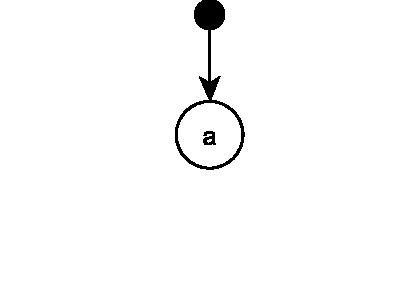
\includegraphics[width=\linewidth]{statechart_01}
        \caption{non-conflict}
        \label{fig:statechart_01}
    \end{subfigure}
    \hfill
    \begin{subfigure}[t]{0.30\linewidth}
        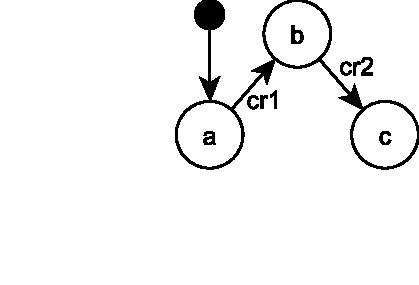
\includegraphics[width=\linewidth]{statechart_02}
        \caption{non-conflict}
        \label{fig:statechart_02}
    \end{subfigure}
    \hfill
    \begin{subfigure}[t]{0.30\linewidth}
        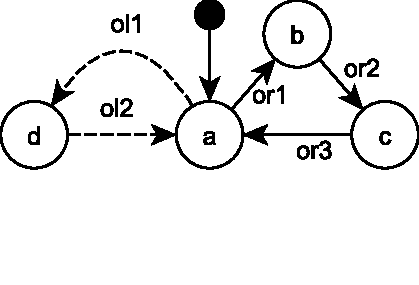
\includegraphics[width=\linewidth]{statechart_03}
        \caption{non-conflict}
        \label{fig:statechart_03}
    \end{subfigure}
    \\
    \begin{subfigure}[t]{0.30\linewidth}
        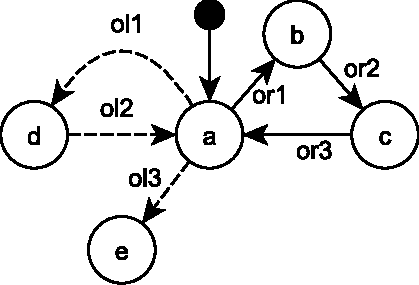
\includegraphics[width=\linewidth]{statechart_04}
        \caption{pseudo-conflict}
        \label{fig:statechart_04}
    \end{subfigure}
    \hfill
    \begin{subfigure}[t]{0.30\linewidth}
        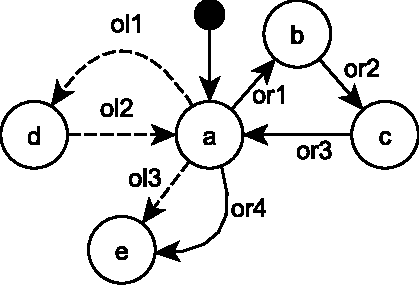
\includegraphics[width=\linewidth]{statechart_05}
        \caption{pseudo-conflict}
        \label{fig:statechart_05}
    \end{subfigure}
    \hfill
    \begin{subfigure}[t]{0.30\linewidth}
        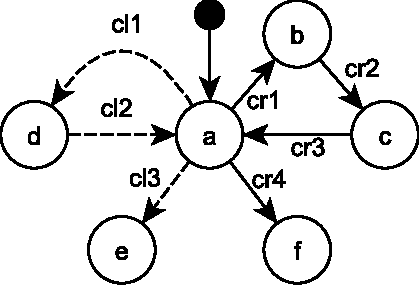
\includegraphics[width=\linewidth]{statechart_06}
        \caption{conflict}
        \label{fig:statechart_06}
    \end{subfigure}
    \caption{Conflicting and non-conflicting change events (dashed arrow = left change event, solid arrow = right change events, circle = state).}
    \label{fig:conflict_states}
\end{figure}

Using (\ref{eq:ecbp_pseudoconflict}), condition in Figure \ref{fig:statechart_04} can be detected as a \textsf{PSEUDO} conflict. \textsf{PSEUDO} conflict means that a conflict can be automatically resolved. This means that we can automatically select one of the two conflicting change event sets as the applied change events without needing for human intervention. Since $C_{R}$ produces the eventual state that is equal to the original state, that is `a'; it does not have any effect -- the changes are not intended or cancelled. Thus, all its change events can be automatically negated. In other words, only change events in $C_{L}$ that are accepted to produce the eventual state, which is `e'. Also using (\ref{eq:ecbp_pseudoconflict}), condition is \ref{fig:statechart_05} can also be detected as another \textsf{PSEUDO} conflict. Both change event sets, $C_{L}$ and $C_{R}$, produce the same eventual state, `e', that is different from the original state, `a'. This condition ca be automatically resolved since selecting one of the sets produces the same outcome. With (\ref{eq:ecbp_conflict}), the condition in Figure \ref{fig:statechart_06} can be detected as a \textsf{REAL} conflict since change event sets, $C_{L}$ and $C_{R}$, produces two different eventual states. The conflict cannot be automatically resolved and requires user intervention to choose which one is the desired eventual state, `e' or `f', and then the appropriate change event set should be selected to produce the eventual state.


\subsection{Conflict Computation} 
\label{sec:conflict_computation} 
We perform procedure in Algorithm \ref{alg:conflict_detection} and employ (\ref{eq:ecbp_conflict}) and (\ref{eq:ecbp_pseudoconflict}) inside it to identify conflicts between two CBPs. Basically, the algorithm works by iterating through all the elements, features, and values in the element three (Figure \ref{fig:right_element_tree_diagram}) and checking the equivalency of their original and eventual states as well the numbers of change events applied to them. The results are then used as inputs to decide whether a conflict has been detected or not.

\begin{table*}[ht]
  \centering
  \caption{Conflicting change events in Listings \ref{lst:cbp_right} and \ref{lst:cbp_left} identified using the proposed conflict detection.}
  \label{table:conflicts_cbp}
  \begin{scriptsize}
    \begin{tabular}{|p{0.04\linewidth}|p{0.38\linewidth}|p{0.38\linewidth}|
        p{0.07\linewidth}|}
      \hline
      \textbf{ID} & 
      \textbf{Left Change Events (Bob)} & 
      \textbf{Right Change Events (Alice)} & 
      \textbf{Type}\\ 
      \hline
      CB1 & 
      set troll.name from "Troll" to "Ogre" & 
      set troll.name from "Troll" to "Orc" & 
      real \\
      \hline
      CB2 & move target in character.parameters from 1 to 2 & 
      move target in character.parameters from 1 to 0 & 
      real \\ 
      \hline
      CB3 & 
      \begin{minipage}[t]{\linewidth}
        \raggedright
        \begin{itemize}[leftmargin=0pt]
          \setlength
          \item[] unset cast.name from "cast" to null
          \item[] remove cast from giant.operations at 0
          \item[] delete cast type Operation
          \item[] unset giant.name from "Giant" to null
          \item[] delete giant
        \end{itemize}
      \end{minipage}
      & 
      \begin{minipage}[t]{\linewidth}
        \raggedright
        \begin{itemize}[leftmargin=0pt]
          \setlength
          \item[] remove cast from giant.operations at 0
          \item[] add cast to mage.operations at 0
          \item[] remove smash from knight.operations at 0
          \item[] add smash to giant.operations at 1
        \end{itemize}
      \end{minipage}
      & 
      real, dependency\\ 
      \hline
      CB4 & 
      set character.name from "Character" to "Hero" & 
      set character.name from "Character" to "Hero" & 
      pseudo\\ 
      \hline
    \end{tabular}
  \end{scriptsize}
\end{table*}

%------------------------------------------------------------------------------

\IncMargin{1.5em}
\begin{algorithm}[ht]
  \begin{scriptsize}
    \SetKwInOut{Input}{input}
    \SetKwInOut{Output}{output}
    \Input{an instance of ElementTree $elementTree$}
    \Begin{
      $conflictList$ $\leftarrow$ ConflictList()\;
      \ForEach{$element$ \In $elementTree$}{
        \tcp{Handle conflicts with deletion ----------------------------}
        \If{isLeftDeleted($element$) \Or isRightDeleted($element$)}{
          $leftEvents$ $\leftarrow$ getAllRelatedLeftEvents($element$)\;
          $rightEvents$ $\leftarrow$ getAllRelatedRightEvents($element$)\;
          \If{size($leftEvents$) > 0 \AndA size($rightEvents$) > 0}{
            $conflict$ $\leftarrow$ createConflict($leftEvents$, $rightEvents$)\;
            \If{isLeftDeleted($element$) \AndA isRightDeleted($element$)}{
              setPseudo($conflict$)\;
            }
            addConflict($conflict$, $conflictList$)\;
          }
        }
        \tcp{Handle conflicts with cross-container move --------------------------}
        \If{(getOriginalContainer($element$) <> getLeftContainer($element$) \Or getOriginalContainingFeature($element$) <> getLeftContainingFeature($element$)) \Or
          (getOriginalContainer($element$) <> getRightContainer($element$) \Or getOriginalContainingFeature($element$) <> getRightContainingFeature($element$))}{
          $leftEvents$ $\leftarrow$ getAllRelatedLeftEvents($element$)\;
          $rightEvents$ $\leftarrow$ getAllRelatedRightEvents($element$)\;
          \If{size($leftEvents$) > 0 \AndA size($rightEvents$) > 0}{
            $conflict$ $\leftarrow$ createConflict($leftEvents$, $rightEvents$)\;
            \If{getLeftContainer($element$) = getRightContainer($element$) \AndA getLeftContainingFeature($element$) = getRightContainingFeature($element$}{
              setPseudo($conflict$)\;
            }
            addConflict($conflict$, $conflictList$)\;
          }
        }
        \ForEach{$feature$ \In getFeatures($element$)}{
          \tcp{Handle single-valued feature --------------------------}
          handleSingleValuedFeature($element$, $feature$, $conflictList$)\;\label{line:conflict_single_value}
          \tcp{Handle multi-valued feature --------------------------} 
          handleMultiValuedFeature($element$, $feature$, $conflictList$)\;\label{line:conflict_multi_value}
        }
      }
      \Return{$conflictList$}\;
    }
  \end{scriptsize}
  \caption{Algorithm for conflict detection using element tree.}
  \label{alg:conflict_detection}
\end{algorithm}
\DecMargin{1.5em}

The algorithm starts by creating a empty list \textsf{conflictList} to contain identified conflicts at lines 2. The algorithm then iterates through all the elements, features, and values in the element three. 

\subsubsection{Conflict with Deletion} 
\label{sec:delete_conflict} 
At lines 4 to 11 in Algorithm \ref{alg:conflict_detection}, the algorithm checks if there is a conflict related to a deletion of an element.
If an element is deleted on one side or both sides, it means that all events related to the element on both sides should be in conflict. 
To get all the related events, the algorithm use functions \textsf{getAllRelatedLeftEvents($element$)} 
and \textsf{getAllRelatedLeftEvents($element$)} (the element acts as a map key to access the change events) that return two sets of the related events, 
\textsf{leftEvents} and \textsf{rightEvents} respectively. The related events are events applied to the deleted element, including its sub-elements and features, 
and events that are parts of composite events. If both sets of events are not empty then a conflict is created containing both sets of events. 
If the element is deleted on both sides then we set the conflict as \textsf{PSEUDO}. The identified conflict is then added to \textsf{conflictList}.

As an example, when the iteration reach element \textsf{giant} in Figure \ref{fig:right_element_tree_diagram}, the algorithm identifies that the element has been deleted only on the left side.
The algorithm then collects all the related events from both sides of the element. 
The left events are all events parts of the composite event that deletes the element. 
The right events consist of events that move operation \textsf{smash} from class \textsf{knight} to class \textsf{giant} and events that
move operation \textsf{cast} from class \textsf{giant} to class \textsf{mage}. The algorithm then creates a conflict that consists of these events 
producing conflict \textsf{CB3} in Table \ref{table:conflicts_cbp}. The conflict is not set \textsf{PSEUDO} since, besides deleted on the left side, its feature also has been modified on the right side. 

\subsubsection{Conflict between Cross-container Moves} 
\label{sec:move_conflict} 
Lines 15 to 25 in Algorithm \ref{alg:conflict_detection} are dedicated to identify conflicts related to cross-container moves. 
First, the algorithm checks if an element has been moved from its original container to another container, on one of the sides or both sides. 
If only on one side or both sides the element has been moved to another container, 
it continues to check the number of events related to the element by firstly obtaining change events related to the element on 
both sides using functions \textsf{getAllRelatedLeftEvents($element$)} and \textsf{getAllRelatedLeftEvents($element$)} yielding two sets of events, 
\textsf{leftEvents} and \textsf{rightEvents}. If the element has, at least, one event on each side,
a conflict is created containing \textsf{leftEvents} and \textsf{rightEvents}. 
If on both sides the element is moved to a same container or the element is moved but finally returns to its original container on one of its sides then the conflict is set to \textsf{PSEUDO}. The conflict is then added to \textsf{conflictList}. 

\subsubsection{Single-valued Feature Conflict} 
\label{sec:single_valued_conflict}
Conflicts that involve single-valued features are handled by the procedure at line \ref{line:conflict_single_value} in Algorithm \ref{alg:conflict_detection}, which is elaborated in Algorithm \ref{alg:conflict_single_valued_feature}. The procedure starts by retrieving \textsf{leftValue}, \textsf{rightValue}, and \textsf{originalValue} of a single-valued feature. It then checks the inequality of \textsf{leftValue} and \textsf{rightValue} to \textsf{originalValue}. If one of \textsf{leftValue} and \textsf{rightValue} are not equal to \textsf{originalValue}, it then continues to check the number of change events related to the feature by firstly retrieving them using functions \textsf{getAllRelatedEvents($element$, $feature$)} and \textsf{getAllRelatedRightEvents($element$, $feature$)} (element and feature act as a map key to access the events) yielding two sets of related events, \textsf{leftEvents} and \textsf{rightEvents}. If \textsf{leftEvents} and \textsf{rightEvents} are not empty then a conflict that contains these events is instantiated. The procedure then checks the equality of \textsf{leftValue} and \textsf{rightValue} and set the conflict to \textsf{PSEUDO} if \textsf{leftValue} and \textsf{rightValue} are equal or one of them is equal to \textsf{originalValue}. Finally, the conflict is put into \textsf{conflictList}. 

\IncMargin{1.5em}
\begin{algorithm}[ht]
  \begin{scriptsize}
    \SetKwInOut{Input}{input}
    \SetKwInOut{Output}{output}
    \Input{an element $element$}
    \Input{a feature $feature$}
    \Input{a list to contain conflicts $conflictList$}
    \Begin{
      \tcp{Handle single-valued feature --------------------------}
      \If{isSingleValued($feature$)}{
        $originalValue$ $\leftarrow$ getOriginalValue($feature$)\;
        $leftValue$ $\leftarrow$ getLeftValue($feature$)\;
        $rightValue$ $\leftarrow$ getRightValue($feature$)\;
        $leftEvents$ $\leftarrow$ getAllRelatedLeftEvents($element$, $feature$)\;
        $rightEvents$ $\leftarrow$ getAllRelatedRightEvents($element$, $feature$)\;
        \If{$originalValue$ <> $leftValue$ \Or $originalValue$ <> $rightValue$ \AndA size($leftEvents$) > 0 \AndA size($rightEvents$) > 0}{
          $conflict$ $\leftarrow$ createConflict($leftEvents$, $rightEvents$)\;
          \If{ $leftValue$ = $rightValue$}{
            setPseudo($conflict$)\;
          }
          addConflict($conflict$, $conflictList$)\;
        }
      }
    }
  \end{scriptsize}
  \caption{Algorithm to handle single-valued feature in conflict detection using element tree -- handleSingleValuedFeature($element$, $feature$, $conflictList$) at line 27 in Algorithm \ref{alg:conflict_detection}.}
  \label{alg:conflict_single_valued_feature}
\end{algorithm}
\DecMargin{1.5em}

For example, when the iteration reach feature \textsf{name} of class \textsf{troll}, the algorithm retrieves the left, right, and original values of the feature, yielding ``Ogre'', ``Orc'', and ``Troll'' respectively. Since ``Ogre'' and Orc'' are not equal to ``Troll'', the algorithm continues to retrieve two sets of events related to the feature. Only one event contained exists in each set. On the left side, the event sets the name of class \textsf{troll} from ``Troll'' to ``Ogre'', while on the right side, the the event sets it from ``Troll'' to ``Orc''. Both event sets are not empty thus a conflict containing them is created. Since ``Ogre'' is not equal to ``Orc'' the conflict is not set to \textsf{PSEUDO}. This conflict is the conflict \textsf{CB1} in Table \ref{table:conflicts_cbp}. This part of the algorithm also identifies conflict \textsf{CB4} except that this conflict is set to \textsf{PSEUDO} since both sides change class \textsf{character}'s \text{name} to ``Hero''.   

\IncMargin{1.5em}
\begin{algorithm}[ht]
  \begin{scriptsize}
    \SetKwInOut{Input}{input}
    \SetKwInOut{Output}{output}
    \Input{an element $element$}
    \Input{a feature $feature$}
    \Input{a list to contain conflicts $conflictList$}
    \Begin{
      \tcp{Handle multi-valued feature --------------------------}
      \If{isMultiValued($feature$)}{
        \uIf{isOrdered($feature$)}{
          $values$ $\leftarrow$ getUnequalLeftAndRightValues($feature$)\;
          \ForEach{$value$ \In $values$}{
            $leftEvents$ $\leftarrow$ getAllRelatedLeftEvents($element$, $feature$, $value$)\;
            $rightEvents$ $\leftarrow$ getAllRelatedRightEvents($element$, $feature$, $value$)\;
            \If{size($leftEvents$) > 0 \AndA size($rightEvents$) > 0}{
              $conflict$ $\leftarrow$ createConflict($leftEvents$, $rightEvents$)\;
              \If{getLeftIndex($value$, $feature$) = getRightIndex($rightValue$, $feature$)}{
                setPseudo($conflict$)\;
              }
              addConflict($conflict$, $conflictList$)\;
            }       
          }
        }\ElseIf{\Not isOrdered($feature$)}{
          $values$ $\leftarrow$ getXORLeftAndRightValues($feature$)\;
          \ForEach{$value$ \In $values$}{
            $leftEvents$ $\leftarrow$ getAllRelatedLeftEvents($element$, $feature$, $value$)\;
            $rightEvents$ $\leftarrow$ getAllRelatedRightEvents($element$, $feature$, $value$)\;
            \If{size($leftEvents$) > 0 \AndA size($rightEvents$) > 0}{
              $conflict$ $\leftarrow$ createConflict($leftEvents$, $rightEvents$)\;
              \If{isExisted($value$, $feature$) = isExisted($rightValue$, $feature$)}{
                setPseudo($conflict$)\;
              }
              addConflict($conflict$, $conflictList$)\;
            }       
          }
        }
      }
    }
  \end{scriptsize}
  \caption{Algorithm to handle multi-valued feature in conflict detection using element tree -- handleMultiValuedFeature($element$, $feature$, $conflictList$) at line 28 in Algorithm \ref{alg:conflict_detection}.}
  \label{alg:conflict_multi_valued_feature}
\end{algorithm}
\DecMargin{1.5em}

\subsubsection{Ordered Multi-valued Feature Conflict} 
\label{sec:ordered_conflict}
Conflicts that involve multi-valued features are handled by the procedure at line \ref{line:conflict_multi_value} in Algorithm \ref{alg:conflict_detection}, which is elaborated in Algorithm \ref{alg:conflict_multi_valued_feature}, where ordered multi-valued features are addressed at lines 3-15. The procedure relies on function \textsf{getUnequalLeftAndRightValues}. The function returns all values from left and right sides that are not equal to their original states in terms of (in)existence and indexes. For example, in Figure \ref{fig:right_element_tree_diagram}, parameter \textsf{target} in feature \textsf{parameters} is at index 2 on the left side but at index 1 in its original state. Thus, the value is included in the returned set. On the right side, this parameter is also at different index to its original index but it is already included the returned set. 

The algorithm then iterates through the values of the set. For each value, it retrieves all events related to the value on this feature (element, feature, and value act as a map key to access the events) using functions \textsf{getAllRelated *Events($element$, $feature$, $value$)}, yielding two sets of events, \textsf{leftEvents} and \textsf{rightEvents}. If both sets of events are not empty then a conflict is created. If the value on both sides is at the same index then the conflict is \textsf{PSEUDO}. Lastly, the conflict is added to \textsf{conflictList}. The parameter \textsf{target} in feature \textsf{parameters} has been concurrently modified; it has one event on each side: parameter \textsf{target} is moved to the last index on the left side and to the first index on the right. Thus, a conflict in detected. This conflict is presented as conflict \textsf{CB2} in Table \ref{table:conflicts_cbp}.

%\begin{figure}[ht]
%    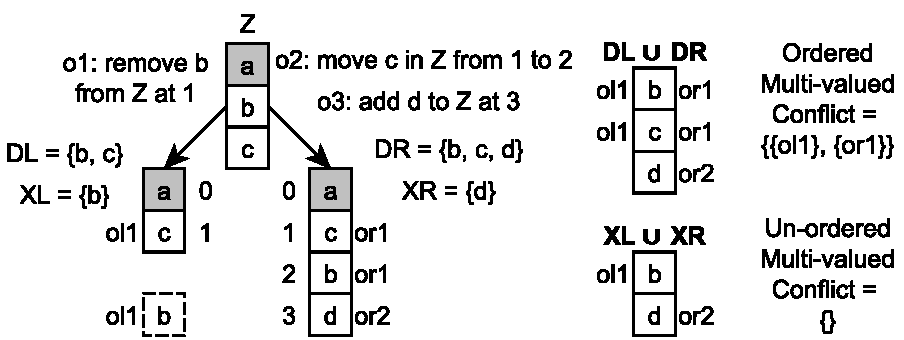
\includegraphics[width=\linewidth]{multi_valued_conflict_detection}
%    \caption{Detecting conflicts in Multi-valued features ($D$: values that are different at every index; $X$: XOR of values).}
%    \label{fig:multi_valued_conflict_detection}
%\end{figure}

\subsubsection{Unordered Multi-valued Feature Conflict} 
\label{sec:unordered_conflict}
Conflict detection for un-odered, multi-valued features is handled at lines 16 to 29 in Algorithm \ref{alg:conflict_multi_valued_feature}. Instead of using function \textsf{getUnequalLeftAndRightValues}, it employs function \textsf{getXORLeftAndRightValues}. The function also returns all values from left and right sides that are not equal to their original states but only in terms of (in)existence since indexing is not important in un-ordered features. The procedure to detect a conflict is similar to the procedure for ordered features. The difference is that, to determine if a conflict is \textsf{PSEUDO} or not, it checks the existence of values (function \textsf{isExisted}).

%\begin{figure*}
%    \begin{tabular}{l|c|r}
%        \begin{subfigure}[t]{0.31\linewidth}
%            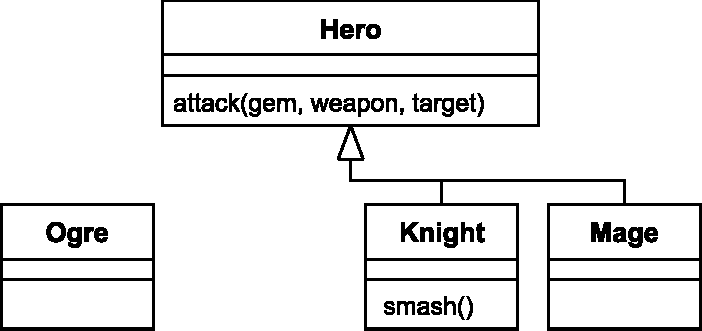
\includegraphics[width=\linewidth]{class_diagram_merged_ecbp}
%            \caption{Epsilon CBP}
%            \label{fig:class_diagram_merged_ecbp}
%        \end{subfigure}
%        &
%        \begin{subfigure}[t]{0.31\linewidth}
%            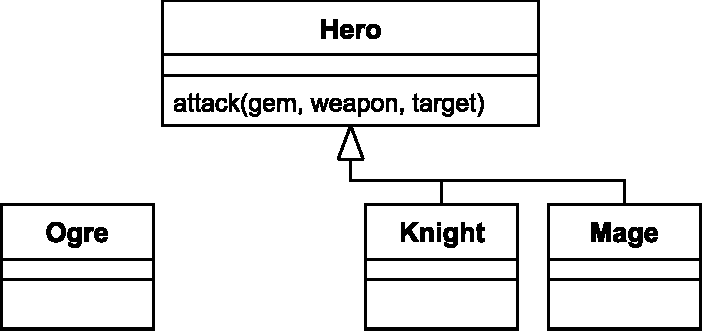
\includegraphics[width=\linewidth]{class_diagram_merged_emfc}
%            \caption{EMF Compare}
%            \label{fig:class_diagram_merged_emfc}
%        \end{subfigure}
%        &
%        \begin{subfigure}[t]{0.31\linewidth}
%            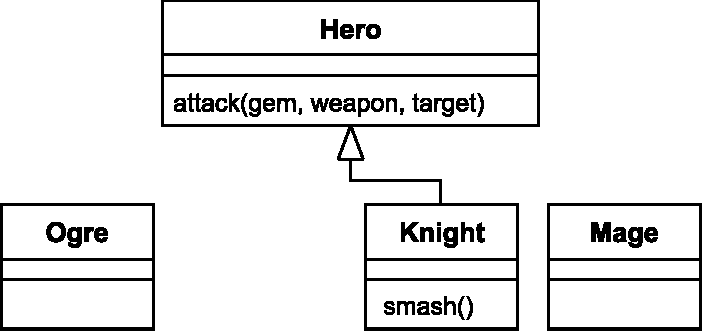
\includegraphics[width=\linewidth]{class_diagram_merged_emfs}
%            \caption{EMF Store}
%            \label{fig:class_diagram_merged_emfs}
%        \end{subfigure}
%    \end{tabular}
%    \caption{Merged models of models in Figure \ref{fig:class_diagram_rpg} after applying all-left-to-right merging.}
%    \label{fig:class_diagram_merged}
%\end{figure*}

%\section{Merging}
%\label{sec:merging}
%Conflict resolution and merging strategies are out of the scope of this paper. However, it is important to present the merged models of these three approaches in order inspect their correctness. Thus, we present the merged models of the models in Figure \ref{fig:class_diagram_rpg} using these three different approaches. The merge is all-left-to-right merge which means the left changes is prioritised above right changes. In other words, the right changes is applied first to the original model so that the left changes can override the right changes. If there is a conflict then the conflicting right changes are cancelled. In EMF Compare, this cancellation means only the left changes are executed, the right changes are \emph{not executed}, while, in Epsilon CBP and EMF Store, the right changes are \emph{reversed} so that the affected elements are brought back to their original states.    
%
%In the default implementation of EMF Compare, the all-left-to-right merge sets the right model as the target and the left model as the source. This means the left changes are not applied to the original model. Instead, they are applied to the right model. Using this strategy, if we resolve all the conflicts in Table \ref{table:conflicts_emfc} using the all-left-to-right merge, we get a merged model as in Figure \ref{fig:class_diagram_merged_emfc}. All the right events are not executed. Instead, in the right model, class \textsf{character}'s feature \text{name} is set to ``Hero'' and class \textsf{troll}'s feature \textsf{name} is set to ``Ogre''. Also, operation \textsf{cast} and class \textsf{giant} are removed from the right model. The removal of class \textsf{giant} also removes operation \textsf{smash} since the operation is contained by the class in the right model. 
%
%For Epsilon CBP and EMF Store, applying the all-left-to-right merging requires all the right events of the conflicts in Tables \ref{table:conflicts_emfs} and \ref{table:conflicts_cbp} to be reversed. This reversal brings back the states of the elements affected by the conflicting right events to their original states which makes the conflicting left events safe to be applied to the original model. All right events are applied first followed by the reversed conflicting right events and then by all left events (see Listings \ref{lst:cbp_merged_emfs} and \ref{lst:cbp_merged_ecbp}). In this order, the events are applied to the original model, not the right model as in the EMF Compare, to produce the merged model.
%
%\begin{lstlisting}[firstnumber=1,style=eol,caption={Merged change events of the models in Figure \ref{fig:class_diagram_rpg} and Listings \ref{lst:cbp_right} and \ref{lst:cbp_left} using EMF Store. The commented lines are added only to improve readability.},label=lst:cbp_merged_emfs]
%#--right events--
%move target in attack.parameters from 1 to 0
%remove smash from knight.operations at 0 composite l1
%add smash to giant.operations at 0 composite l1
%remove cast from giant.operations at 1 composite l2
%add cast to mage.operations at 0 composite l2
%create rightGen type Generalization
%set rightGen.general to character
%set troll.generalization to rightGen
%set character.name from "Character" to "Hero"
%remove rightGen from troll.generalization composite l3
%set mage.generalization to rightGen composite l3
%set troll.name from "Troll" to "Orc"
%#--reversed conflicting right events--
%set troll.name from "Orc" to "Troll"
%remove rightGen from mage.generalization composite l3r
%set troll.generalization to rightGen composite l3r
%set character.name from "Hero" to "Character"
%remove rightGen from troll.generalization
%set rightGen.general from character to null
%delete rightGen
%remove cast from mage.operations at 0 composite l2r
%add cast to giant.operations at 1 composite l2r
%remove smash from giant.operations at 0 composite l1r
%add smash to knight.operations at 0 composite l1r
%move target in attack.parameters from 0 to 1
%#--left events--
%create leftGen type Generalization
%set leftGen.general to character
%set troll.generalization to leftGen
%set character.name from "Character" to "Hero"
%remove leftGen from troll.generalization composite r1
%set knight.generalization to leftGen composite r1
%move target in attack.parameters from 1 to 2
%unset cast.name from "cast" to null composite r2
%remove cast from giant.operations at 0 composite r2
%delete cast composite r2
%unset giant.name from "Giant" to null composite r2
%delete giant comp r2
%set troll.name from "Troll" to "Ogre"
%\end{lstlisting}
%
%\vspace{-20pt}
%\begin{lstlisting}[firstnumber=1,style=eol,caption={Merged change events (operations) of the models in Figure \ref{fig:class_diagram_rpg} and Listings \ref{lst:cbp_right} and \ref{lst:cbp_left} using Epsilon CBP. The commented lines are added only to improve readability.},label=lst:cbp_merged_ecbp]
%#--right events--
%move target in attack.parameters from 1 to 0
%remove smash from knight.operations at 0 composite l1
%add smash to giant.operations at 0 composite l1
%remove cast from giant.operations at 1 composite l2
%add cast to mage.operations at 0 composite l2
%create rightGen type Generalization
%set rightGen.general to character
%set troll.generalization to rightGen
%set character.name from "Character" to "Hero"
%remove rightGen from troll.generalization composite l3
%set mage.generalization to rightGen composite l3
%set troll.name from "Troll" to "Orc"
%#--reversed conflicting right events--
%set troll.name from "Orc" to "Troll"
%remove cast from mage.operations at 0 composite l2r
%add cast to giant.operations at 1 composite l2r
%remove smash from giant.operations at 0 composite l1r
%add smash to knight.operations at 0 composite l1r
%move target in attack.parameters from 0 to 1
%#--left events--
%create leftGen type Generalization
%set leftGen.general to character
%set troll.generalization to leftGen
%set character.name from "Character" to "Hero"
%remove leftGen from troll.generalization composite r1
%set knight.generalization to leftGen composite r1
%move target in attack.parameters from 1 to 2
%unset cast.name from "cast" to null composite r2
%remove cast from giant.operations at 0 composite r2
%delete cast composite r2
%unset giant.name from "Giant" to null composite r2
%delete giant comp r2
%set troll.name from "Troll" to "Ogre"
%\end{lstlisting}
%
%The drawback of the EMF Compare approach is that it set the right model as the target for merging changes resulting the lost of operation \textsf{smash} in the merged model (Figure \ref{fig:class_diagram_merged_emfc}). In contrast, Epsilon CBP and EMF Store reverse the event that moves operation \textsf{smash} from class \textsf{knight} to class \textsf{giant} so that it moves back operation \textsf{smash} from class \textsf{giant} to class \textsf{knight}. The drawback of EMF Store is that it does not concern about the eventual states produced by the conflicting events. It only concern that a feature has been modified concurrently on both sides identified by the presence of, at least, an event on each side. For example, the eventual states of class \textsf{troll}'s feature \textsf{generalization} are \textsf{null} in the original, left, and right models. However, these are not considered by EMF Store. Instead, it only identifies that there are events on both sides associated to this feature. Thus, conflict \textsf{ES1} in \ref{table:conflicts_emfs} is generated. In consequence, all events related to the feature on the right side, and the events that are part of their composite events, are reversed resulting the exclusion of generalization \textsf{rightGen} from the merged model. This drawback has been addressed by the Epsilon CBP by checking the equality of the original, left, and right states of the feature. Since they are all equal then there is no conflict between the events. Thus, Epsilon CBP produces a merged model as in Figure \ref{fig:class_diagram_merged_ecbp}.


\section{Evaluation Method}
\label{sec:evaluation_conflict_Detection}
This section presents the method that was employed to evaluate the change-based conflict detection approach proposed in this study and discuss the results. In order to assess the performance benefits of the proposed conflict detection, this study has evaluated it against a mature and widely-used state-based model comparison tool, EMF Compare \cite{emfcompare2018developer,eclipse2017compare}, and another implementation of change-based model persistence, EMF Store \cite{koegel2010emfstore}. EMF Store is not included in the model differencing evaluation in Chapter \ref{ch:model_differencing} since it works purely on changes, and it is designed to identify conflict between changes; not for finding differences between models. 

Since there are no manually developed, large models persisted in the proposed change-based format yet, the dataset for this experiments was constructed from a large model reverse-engineered from the Eclipse Epsilon project \cite{eclipse2018epsilongit,eclipse2017epsilon}. This model conforms to the Java metamodel \cite{eclipse2018modiscojava} and consists of more than 1.6 million elements with a size of 224 MBs when persisted in XMI. 

The original model was cloned to produce two new (left and right) models and perform operations (\textsf{add}, \textsf{remove}, \textsf{move}, \textsf{set} with random elements, features, indexes, and values) on both models to create differences. In the evaluation, 1.1 million artificial changes were applied to each model, generating over 1.1 million events (one operation can generate more than one event, e.g. a \textsf{move} between features generates \textsf{remove} and \textsf{add} events). Events generated by the changes were persisted in the proposed change-based format (to be used later in change-based model comparison). After every 50,000 changes, a measurement point is made. The eventual state of the models were persisted in state-based format (to be used later in state-based model comparison) and then conflict detection using EMF Compare, EMF Store, and Epsilon CBP were performed and their execution time and memory footprint were measured. In one experiment, 22 measurement points to capture their trends. For EMF Store, the changes persisted in Epsilon CBP format were imported into EMF Store by replaying them in the EMF Store; equivalent changes could be obtained but executed on EMF Store. 

This evaluation conducted five experiments to evaluate the model conflict detection of the proposed approach. In the first experiment, the ratio of occurrence between \textsf{add}, \textsf{remove}, \textsf{move}, and \textsf{set} changes is set to 1:1:20:40 intuitively in assumption that in a mature model modification -- \textsf{move} and \textsf{set} events -- occurs more frequent than addition and deletion. To reduce the effect of the change on the number of total elements to our measurement, the number of total elements should be kept constant. For example, it is difficult to tell an increase of time in comparison is caused by an increase in the number of elements or by the number of change events. One way to do this was to exclude \textsf{add} and \textsf{remove} operations. However, excluding both operations made measurement less representative. Thus, both operations were still included but their probabilities were made equal so that the number of total elements remain largely unchanged. In the rest of the experiments,
homogeneous type change events -- isolated from other types -- were performed per experiment (e.g. add-only, move-only change events). In the end, 5 results of the experiments were obtained: mixed, add-only, remove-only, move-only, and set-only measurement results. They are useful to asses whether operations of different types have a different impact on model comparison. For the delete-only experiment on EMF Store, due to slow execution of replaying \textsf{delete} event in EMF Store, the size of the models was reduced from 1.6 million to only 70 thousand elements each, and the number of changes from 1.1 millions to 550 thousands with 25 thousand changes for each measurement point, still 22 measurement points in total.

For conflict detection in Epsilon CBP, the conflict detection time comprises loading change events, constructing an element tree, and computing conflicts. The memory footprint is the space used to hold the change events, element tree, and conflicts in memory. For EMF Compare, the comparison time comprises matching elements and identifying differences, and the memory footprint is the space required to hold the matches and differences in memory. For EMF Store, the conflict detection time comprises loading and mapping change events and computing conflicts. The memory footprint is the space used to hold the change events and mapping and conflicts in memory.

All measurements were performed on the same machine with the following specification: AMD Opteron(tm) Processor 6386 SE @ 2.8 GHz cache size 2 GBs (64 processors), 528 GBs main memory, Ubuntu 16.04.6 LTS operating system, and Java(TM) SE Runtime Environment (build 1.8.0\_201-b09) with JVM \textsf{InitialHeapSize} 2GBs and \textsf{MaxHeapSize} 32 GBs.

%Since the change-based and state-based approaches can produce a different number of syntactically equivalent differences, in order to evaluate the correctness of the change-based approach, we reconciled all the differences by performing all-left-to-right merging -- making the right model identical to the left model -- based on the identified differences. If the all-left-to-right merging of change-based approach produces a model that is identical to the model produced by the all-left-to-right merging of the state-based approach then it can be said that differences identified by the change-based approach are correct. We performed this correctness checking at every measurement point.

\begin{figure*}[ht]
  \centering
  \begin{subfigure}[t]{0.495\linewidth}
    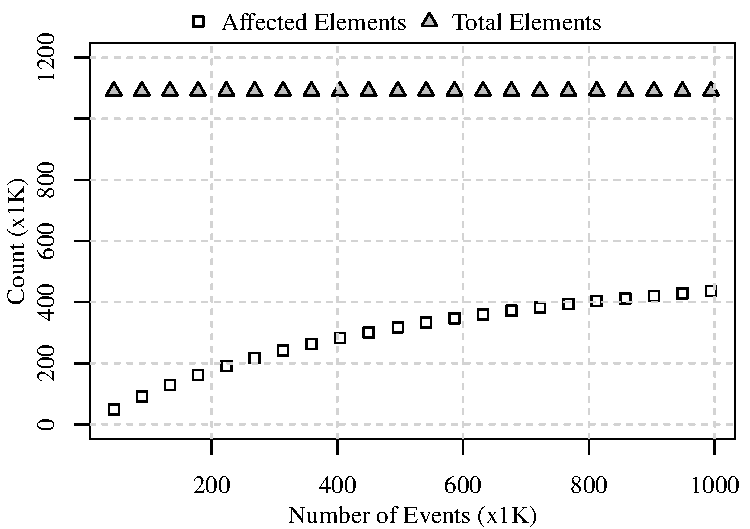
\includegraphics[width=\linewidth]{conflict-size-events}
    \caption{number of elements}
    \label{fig:conflict-size-events}
  \end{subfigure}
  \hfill
  \begin{subfigure}[t]{0.495\linewidth}
    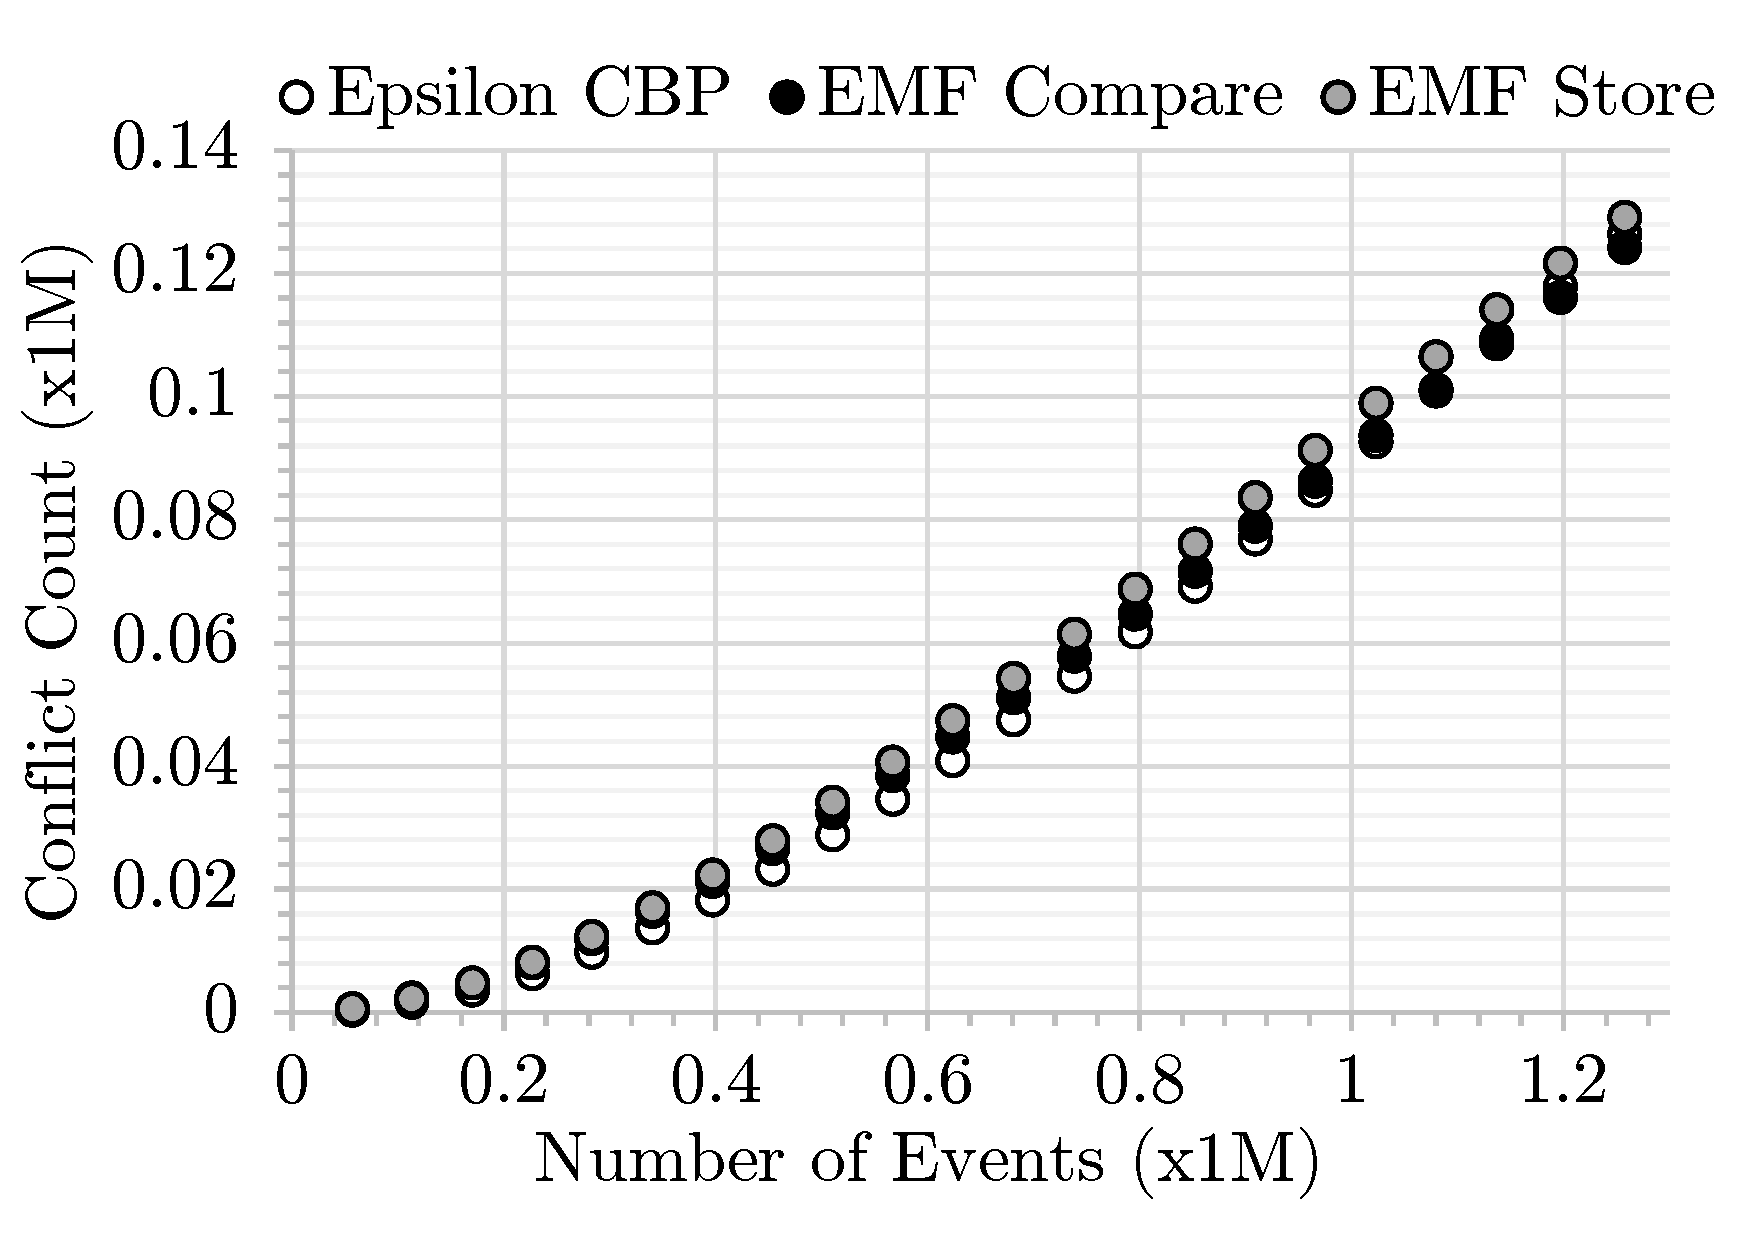
\includegraphics[width=\linewidth]{conflict-count-events}
    \caption{number of conflicts}
    \label{fig:conflict-count-events}
  \end{subfigure}
  \\
  \begin{subfigure}[t]{0.495\linewidth}
    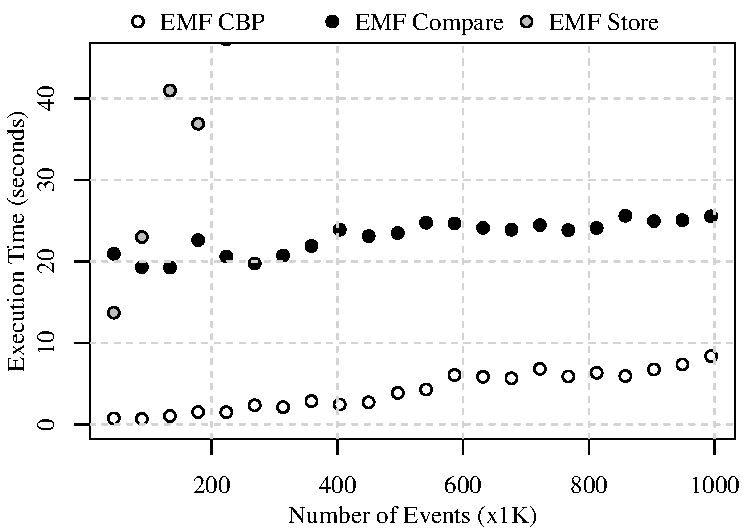
\includegraphics[width=\linewidth]{conflict-time-events}
    \caption{execution time}
    \label{fig:conflict-time-events}
  \end{subfigure}
  \hfill
  \begin{subfigure}[t]{0.495\linewidth}
    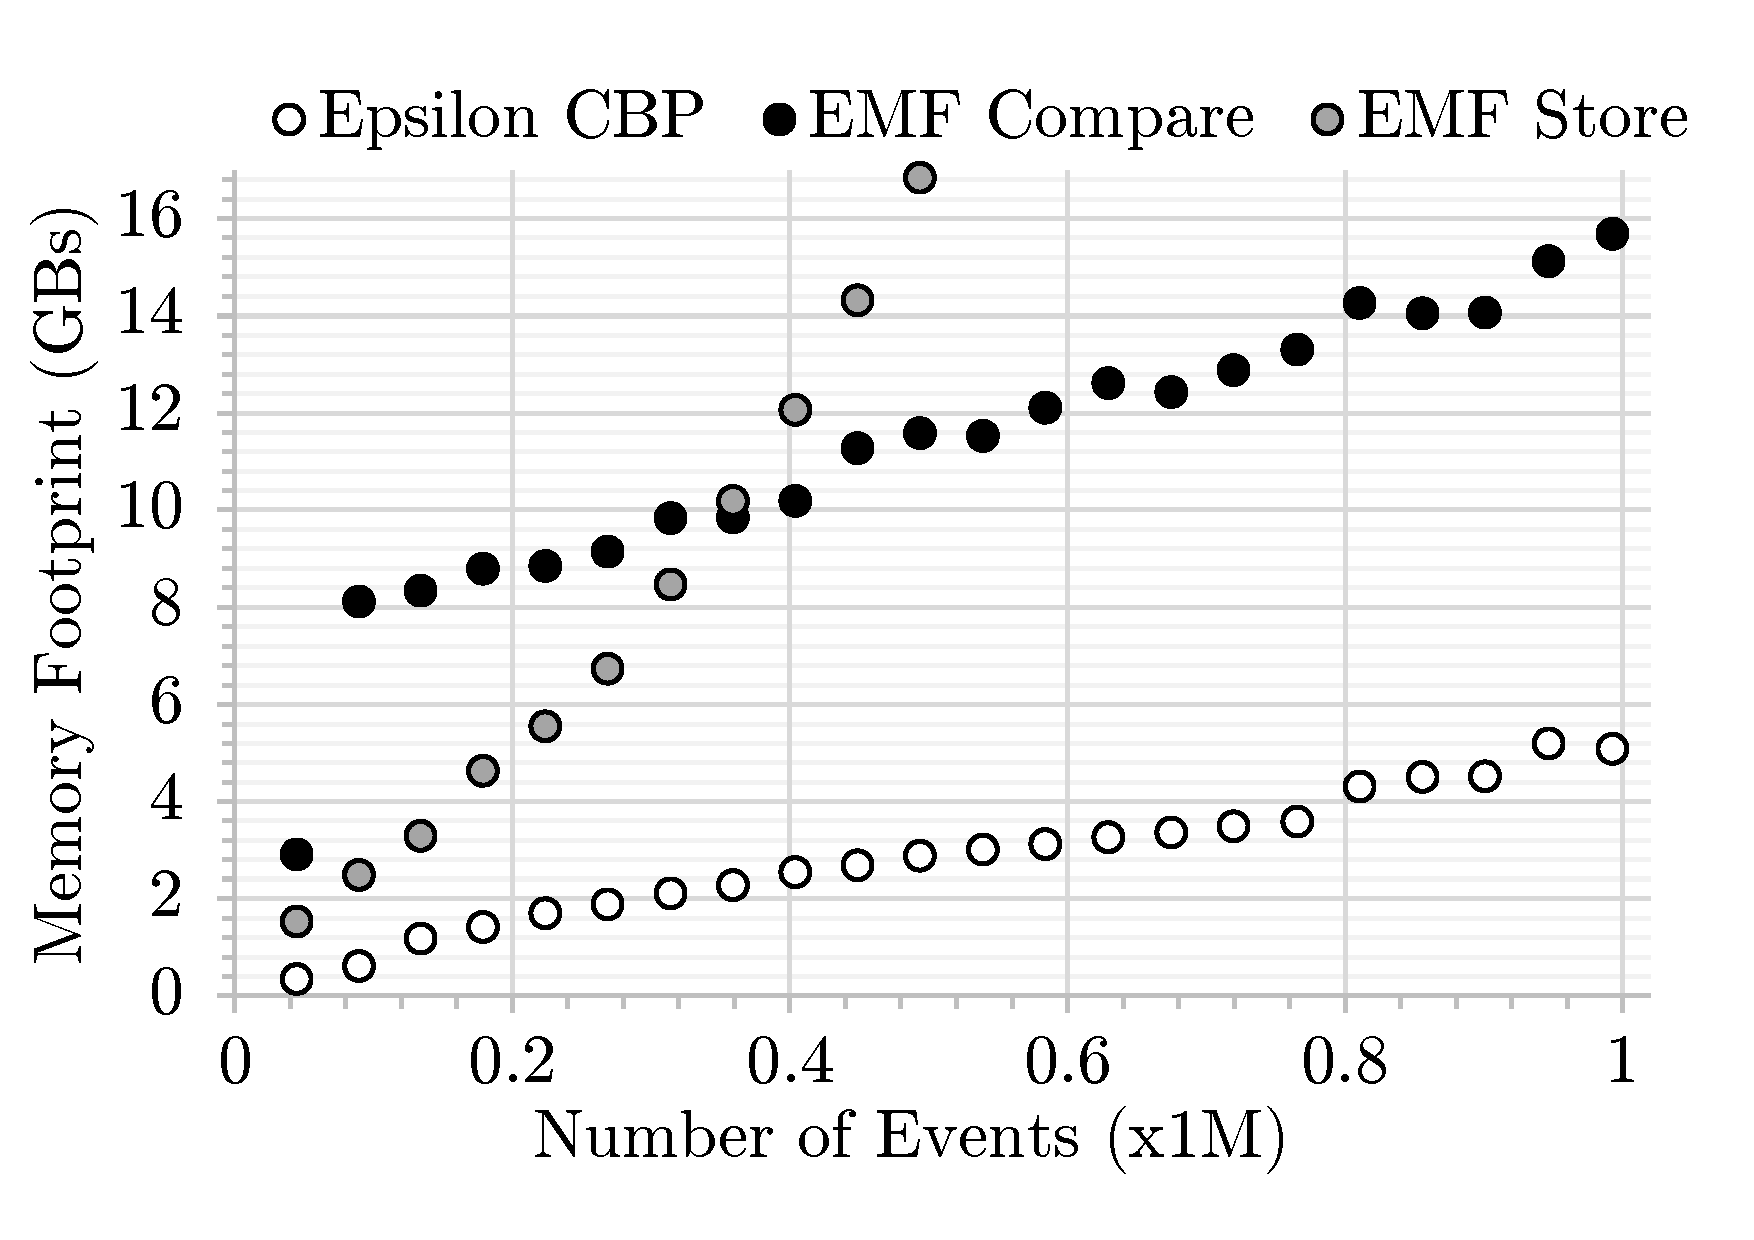
\includegraphics[width=\linewidth]{conflict-memory-events}
    \caption{memory footprint}
    \label{fig:conflict-memory-events}
  \end{subfigure}
  \caption{Epsilon CBP vs. EMF Compare vs. EMF Store comparison as change events increase.}
  \label{fig:conflict_events}
\end{figure*}

\vspace{-5pt}
\section{Evaluation Results and Discussion}
\label{sec:evaluation_discussion}
In this section, we report on the obtained results in terms of comparison time and memory footprint for conflict detection. 

\vspace{-5pt}
\subsection{Mixed Operations}
\label{sec:mixed-operation_conflict}

\begin{wrapfigure}[14]{r}{0.5\textwidth}
  \vspace{-5pt}
  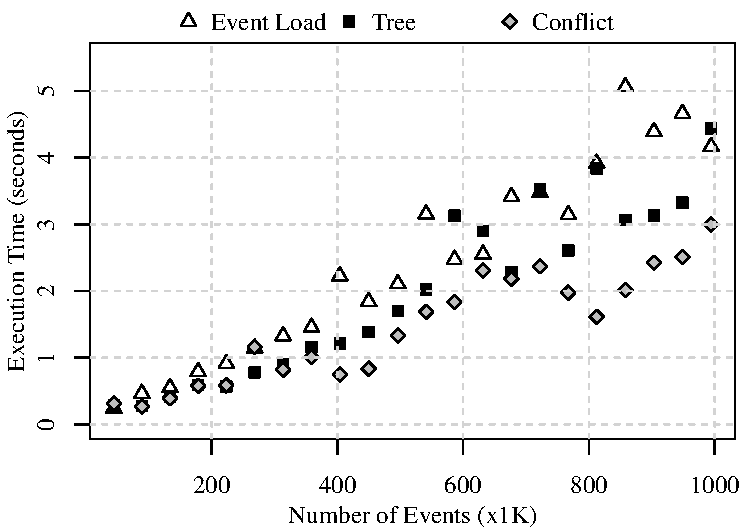
\includegraphics[width=\linewidth]{ecbp-conflict-time-events}
  \caption{A breakdown view of Epsilon CBP on the time required for conflict detection.}
  \label{fig:ecbp-conflict-time-events}
\end{wrapfigure}

In the mixed operation measurement, we modify two identical models differently by applying random operations. As the number of change events generated by the modification grows, the numbers of affected elements and differences also increase in a logarithmic manner. The patterns can be seen in Figure \ref{fig:modification_course}. The growth is logarithmic since the probability that the random operations modify the same elements also increases. Thus, some change events might not contribute to the addition of new affected elements and differences. In other words, more events are required to increase the number of affected elements or differences. In Figure \ref{fig:modification_course}, the total elements remains largely unchanged due to the equal probabilities of addition and deletion as has been set in Section \ref{sec:evaluation}. The figure gives us an insight about the characteristics of the modification caused by the random operations in the mixed operation measurement; it supports explaining the implication of the changes on execution time and memory footprints of model comparison.

\begin{figure}[ht]
  \centering
  \begin{minipage}[b]{0.495\textwidth}
    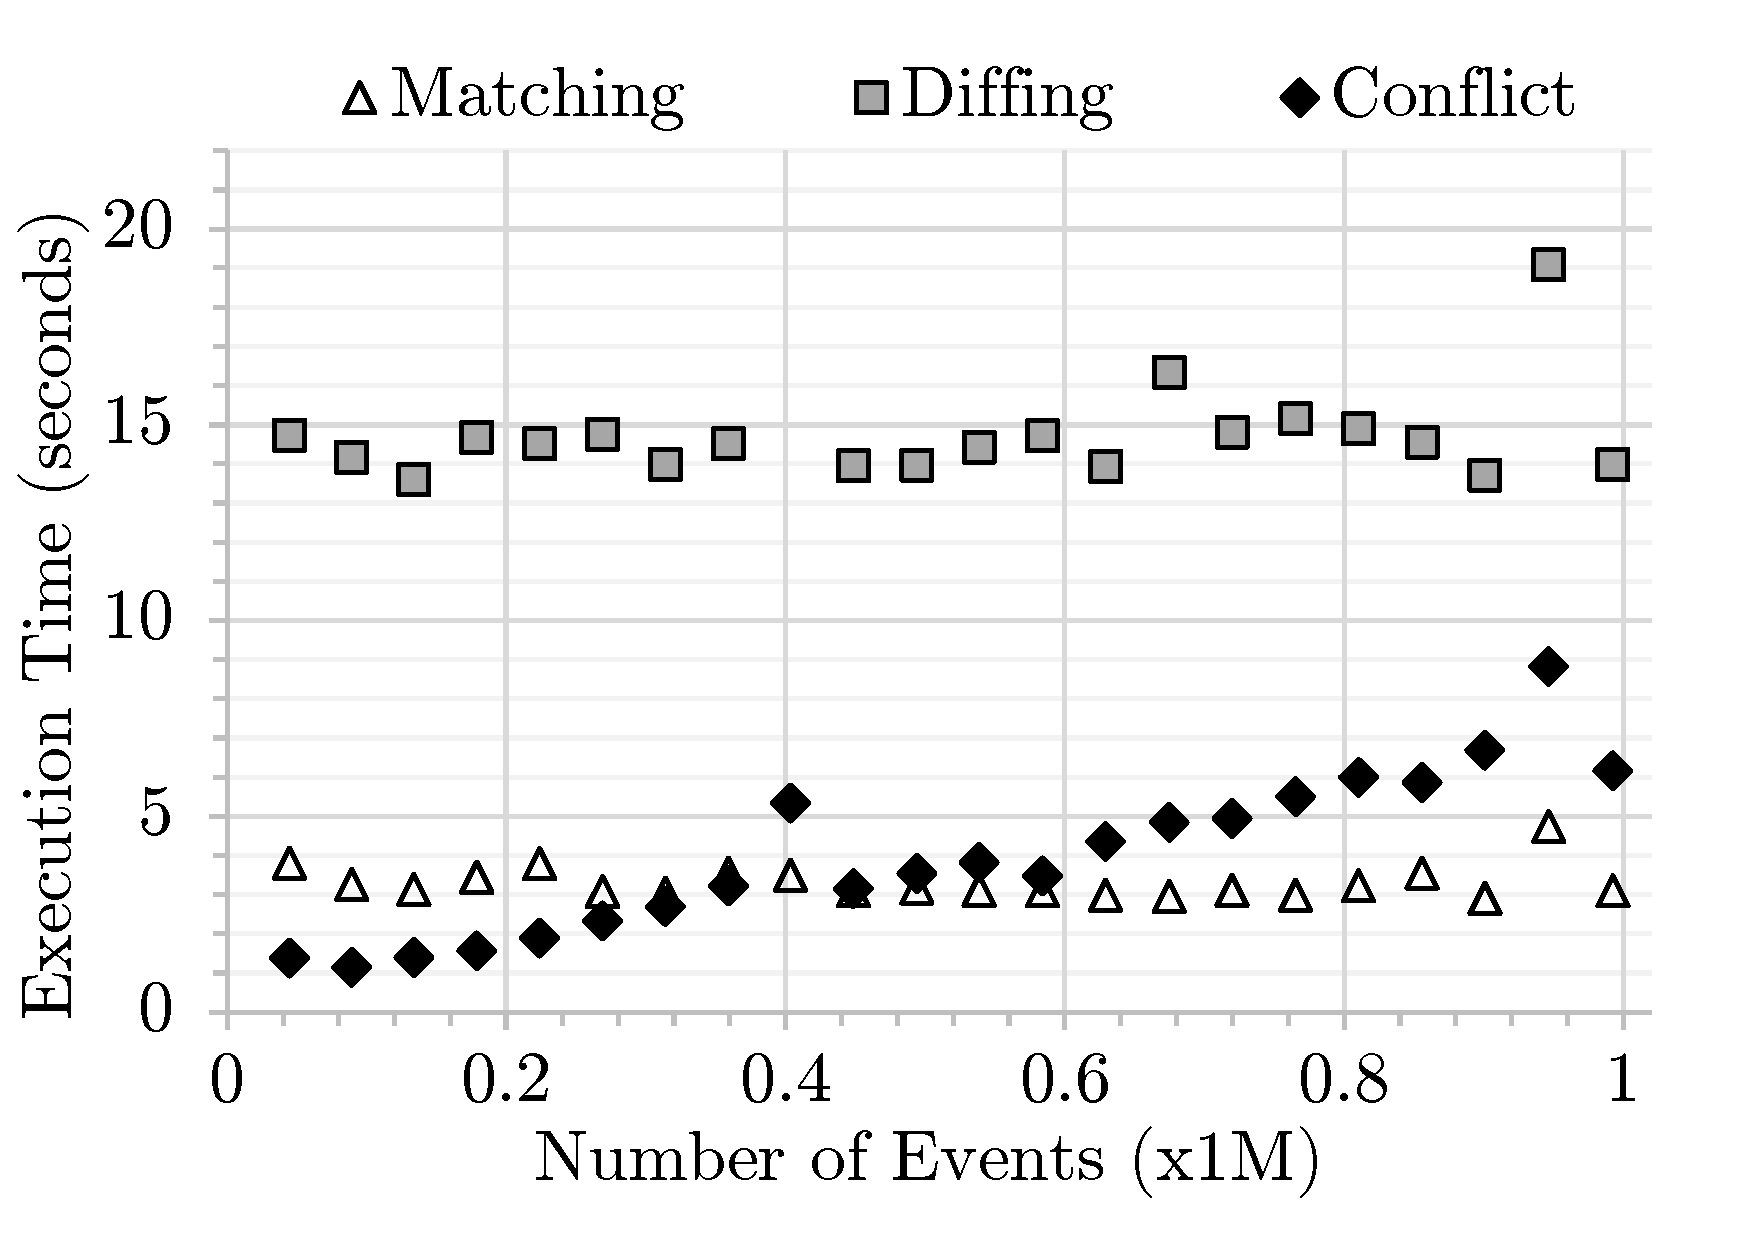
\includegraphics[width=\linewidth]{emfc-conflict-time-events}
    \caption{A breakdown view of EMF Compare on the time required for conflict detection.}
    \label{fig:emfc-conflict-time-events}
  \end{minipage}
  \hfill
  \begin{minipage}[b]{0.495\textwidth}
    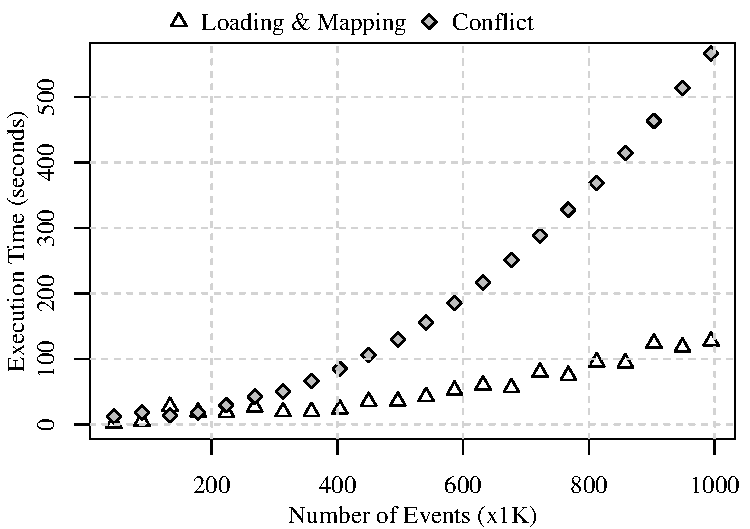
\includegraphics[width=\linewidth]{emfs-conflict-time-events}
    \caption{A breakdown view of EMF Store on the time required for conflict detection.}
    \label{fig:emfs-conflict-time-events}
  \end{minipage}
\end{figure}

Similar to the results in the model differencing evaluation (Figure \ref{fig:modification_course}), the growing number of change events in the conflict detection evaluation is also followed by the logarithmic increase of affected elements (Figure \ref{fig:conflict-size-events}). The total number of both elements can also be kept relatively constant due to 1:1 ratio of \textsf{add} and \textsf{delete} operations' occurrence. These change events produce different numbers of conflicts for Epsilon CBP, EMF Compare, and EMF Store as can be seen in Figure \ref{fig:conflict-count-events}. However, the numbers of conflicts detected are slightly different due to their distinct conflict detection approaches. 

\begin{wrapfigure}[14]{r}{0.5\textwidth}
  \vspace{-7pt}
  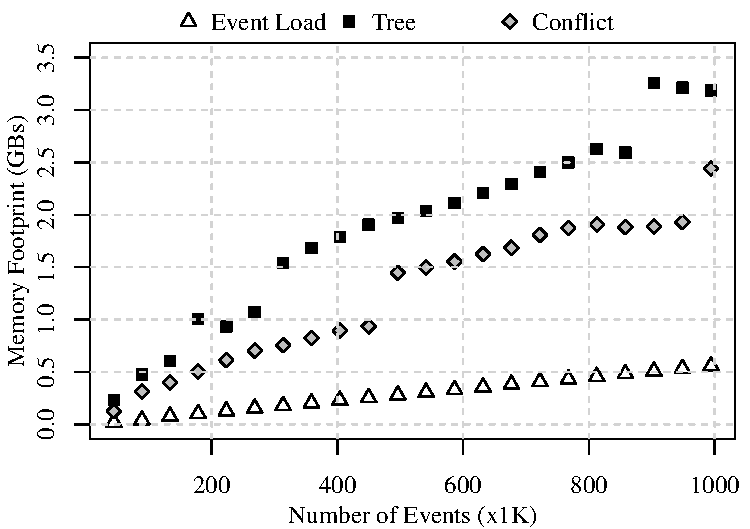
\includegraphics[width=\linewidth]{ecbp-conflict-memory-events}
  \caption{A breakdown view of Epsilon CBP on the memory footprint for conflict detection.}
  \label{fig:ecbp-conflict-memory-events}
\end{wrapfigure}

Figure \ref{fig:conflict-time-events} exhibits Epsilon CBP outperforms EMF Compare and EMF Store in terms of execution time in detecting conflicts. In a comparison of two models that involves 1.01 million elements in total and 1.3 millions change events (the last measurement point), Epsilon CBP takes only 6.7 seconds to detect all conflicts while EMF Compare requires 21.4 seconds to finish the conflict detection. Both conflict detections are faster than EMF Store that needs 1 minute and 34.6 seconds to complete detecting conflicts. Figure \ref{fig:conflict-memory-events} also shows Epsilon CBP outmatches EMF Compare and EMF Store in terms of memory footprint in conflict detection. At the last measurement point, Epsilon CBP only consumes 5 GBs which is much lesser than EMF Compare and EMF Store that occupy around 16 and 26 GBs of memory footprint respectively.

\begin{figure}[ht]
  \begin{minipage}[b]{0.495\textwidth}
    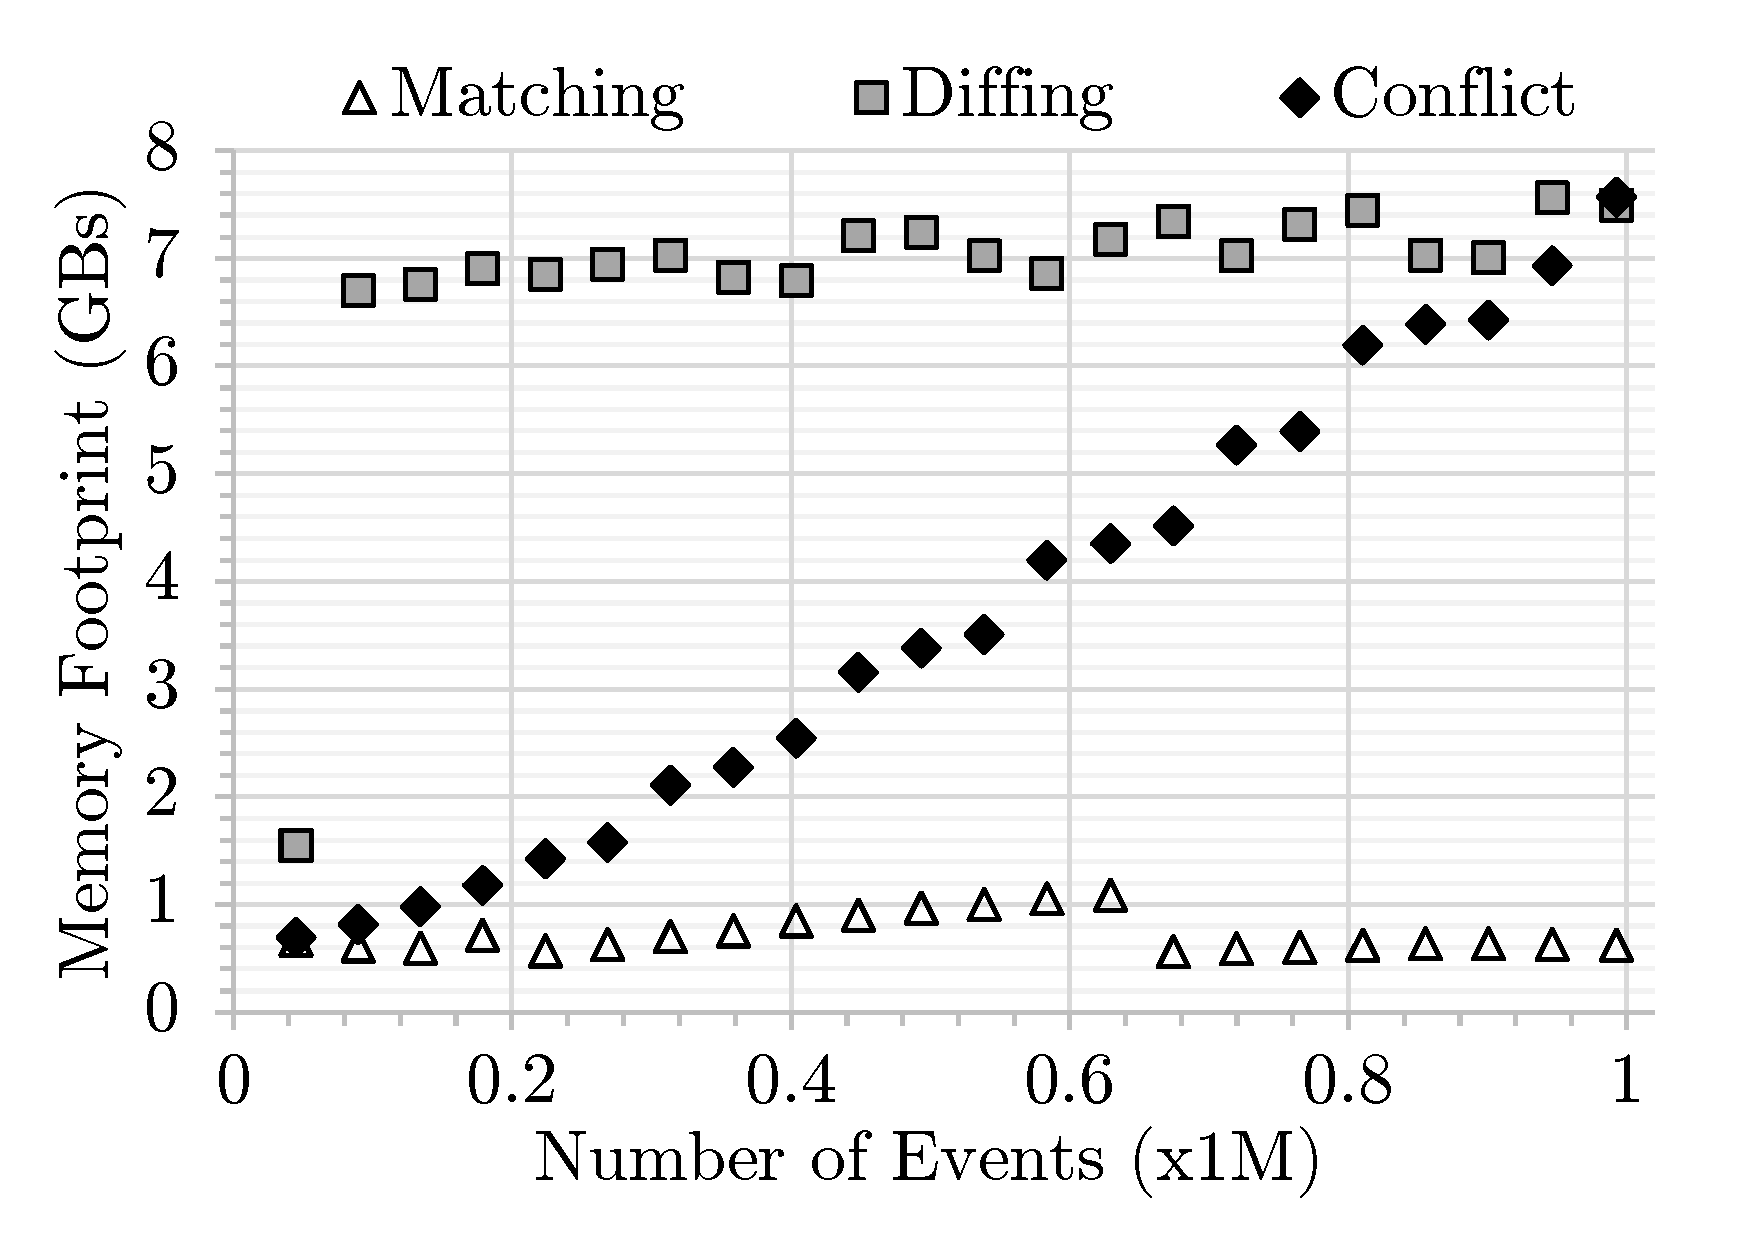
\includegraphics[width=\linewidth]{emfc-conflict-memory-events}
    \caption{A breakdown view of EMF Compare on the memory footprint for conflict detection.}
        \label{fig:emfc-conflict-memory-events}
  \end{minipage}
\hfill
  \begin{minipage}[b]{0.495\textwidth}
    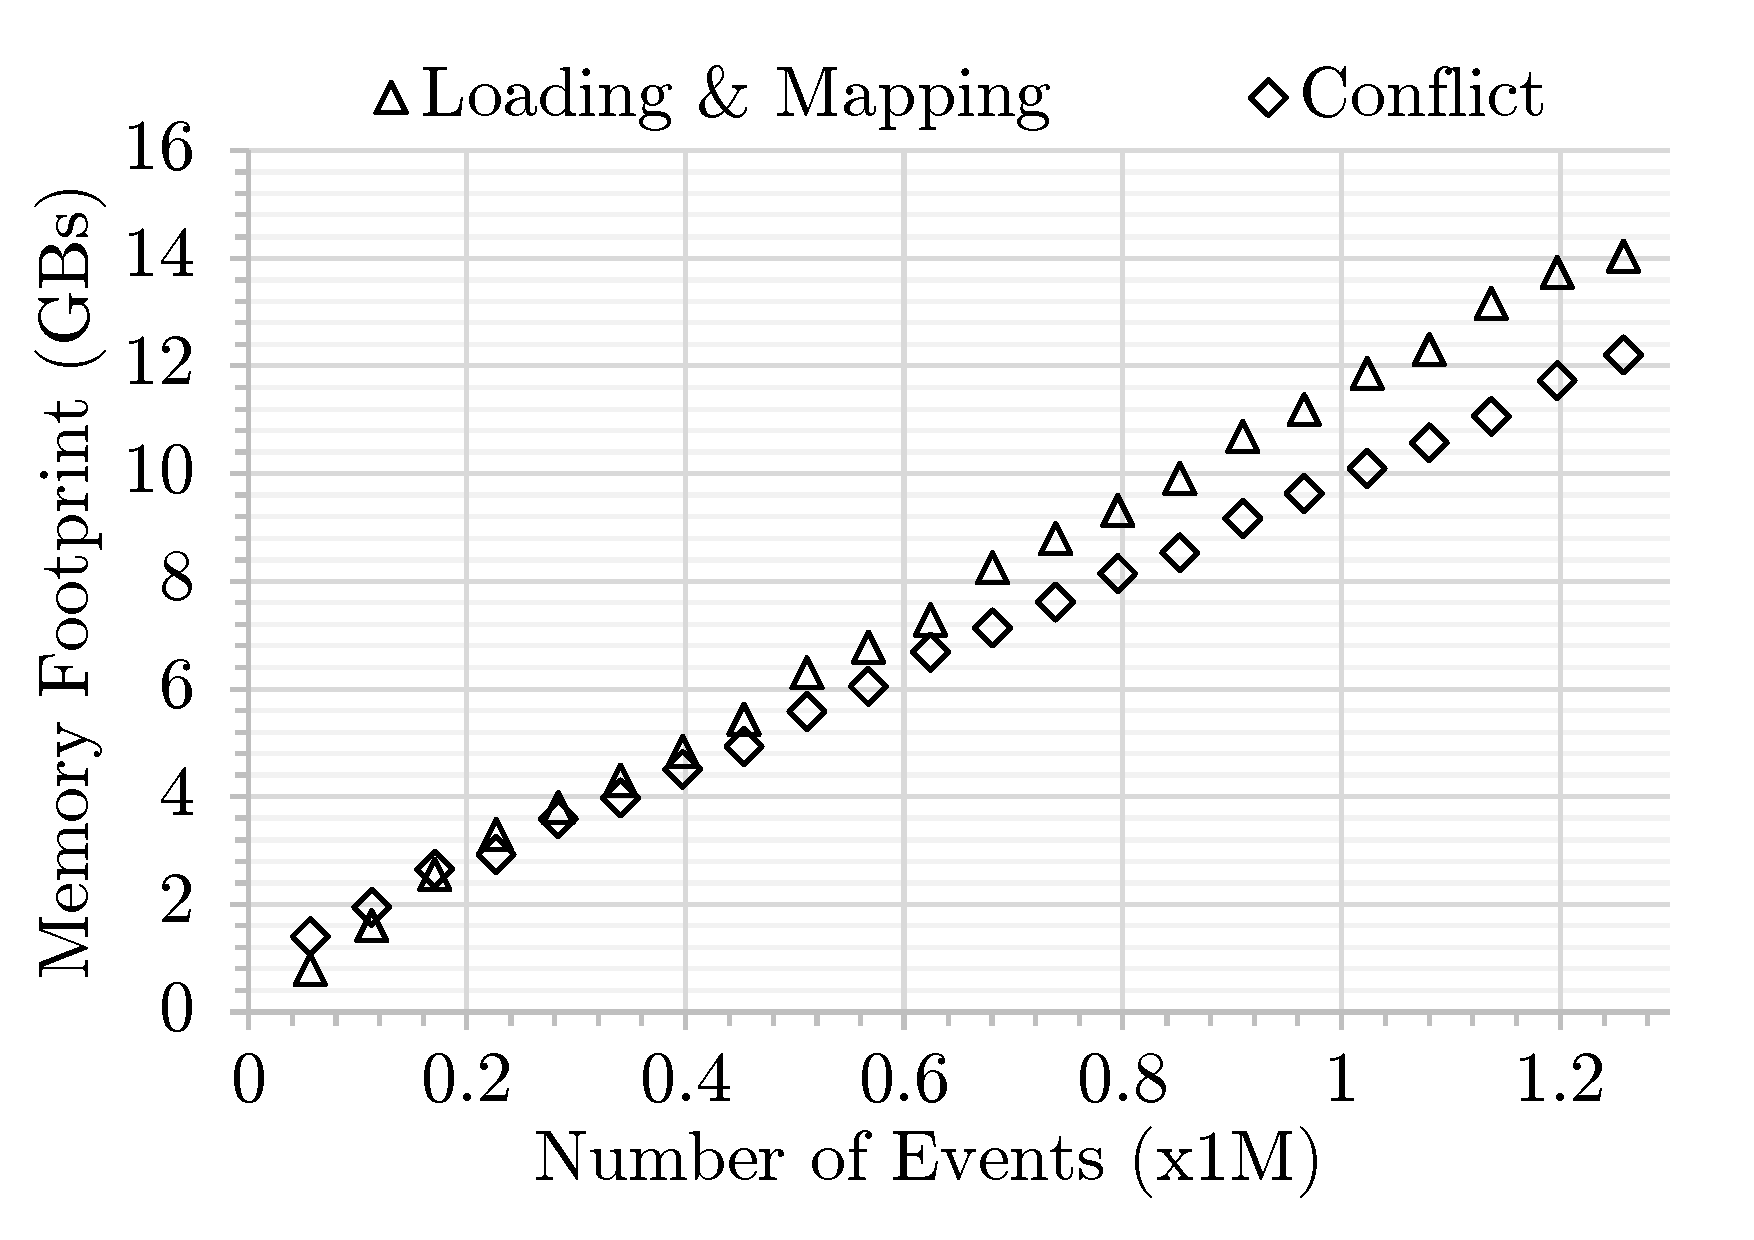
\includegraphics[width=\linewidth]{emfs-conflict-memory-events}
    \caption{A breakdown view of EMF Store on the memory footprint for conflict detection.}
    \label{fig:emfs-conflict-memory-events}
  \end{minipage}
\end{figure}

Figure \ref{fig:conflict-time-events} shows the detailed view of Epsilon CBP, EMF Compare, and EMF Store on the time required to complete conflict detection. As can be seen in the Figure \ref{fig:ecbp-conflict-time-events}, Epsilon CBP takes most of the time used to load change events and construct element tree compared to the time it takes for identifying conflicts. In detecting conflicts, the Epsilon CBP does not requires to perform differencing since changes are already available in the form of change events Thus, the differencing is not included in the diagram. In EMF Compare, at the last measurement point, we can notice that the time taken for matching and identifying conflicts is less than 6 seconds each, which is smaller than the time used for identifying differences that is 12.6 seconds (Figure \ref{fig:emfc-conflict-time-events}). The differencing takes a great portion of the time since it needs to derive differences twice; differences between left and original models and right and original models. The time for for matching and differencing tends to have only slight increase since the sizes of the models are set to be as constant as possible (Figure \ref{fig:modification_course}). In contrast, the time for detecting conflicts tends to grow faster than both due to the increasing number of conflicting (derived) changes as the number of modification -- change events -- increases. In detecting conflicts, EMF Store allocates more than a half of the consumed time for identifying conflicts. The rest of the time is used for loading changes and mapping between affected elements and their ids (Figure \ref{fig:emfs-conflict-time-events}). 

In terms of memory footprint, Epsilon CBP allocates most of the memory space for element tree construction and the rest is for the loading change events and identifying conflicts (Figure \ref{fig:ecbp-conflict-memory-events}). The reason for this is due to our technical implementation explained in Section \ref{sec:mixed-operation}. In EMF Compare (Figure \ref{fig:emfc-conflict-memory-events})), the amount of memory used for matching and differencing only increases slightly due the sizes of the models that are set to be as constant as possible (Figure \ref{fig:modification_course}). In contrast, the memory used for detecting conflict increases positively as the number of detected conflicts rises (Figure \ref{fig:conflict-count-events}). For EMF Store, the amount of memory used for loading changes and mapping is slightly above the amount of memory for identifying differences (Figure \ref{fig:emfs-conflict-memory-events}).

\begin{figure*}[ht]
  \centering
  \begin{subfigure}[t]{0.495\linewidth}
    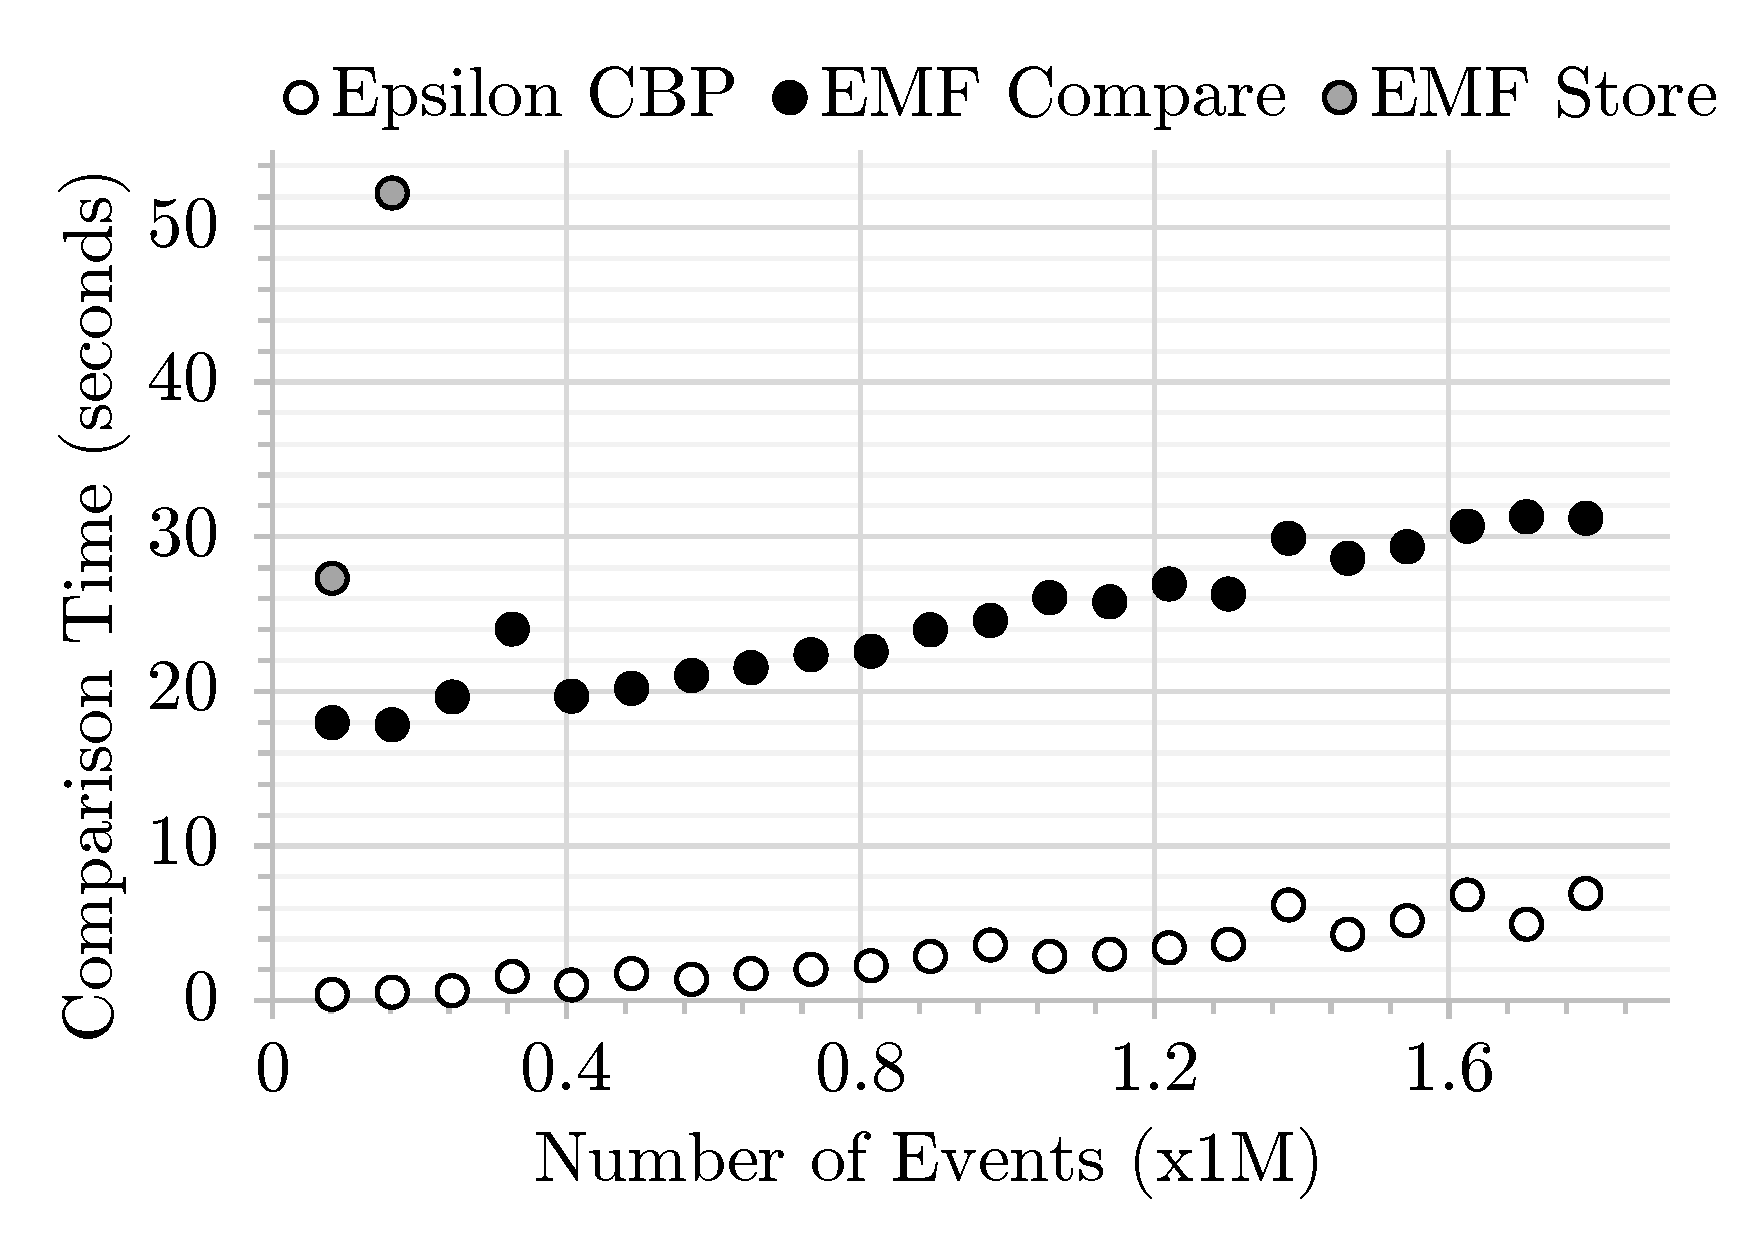
\includegraphics[width=\linewidth]{add-conflict-time-events}
    \caption{add-only}
    \label{fig:add-conflict-time-events}
  \end{subfigure}
  \hfill
  \begin{subfigure}[t]{0.495\linewidth}
    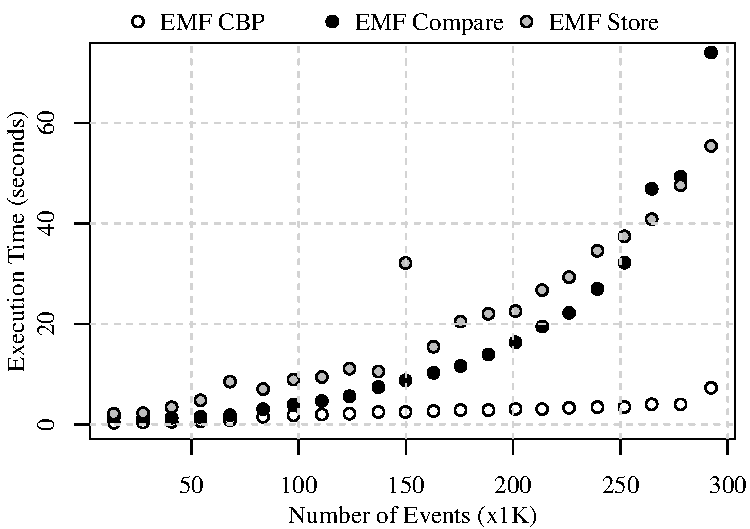
\includegraphics[width=\linewidth]{delete-conflict-time-events}
    \caption{delete-only}
    \label{fig:delete-conflict-time-events}
  \end{subfigure}
  \\
  \begin{subfigure}[t]{0.495\linewidth}
    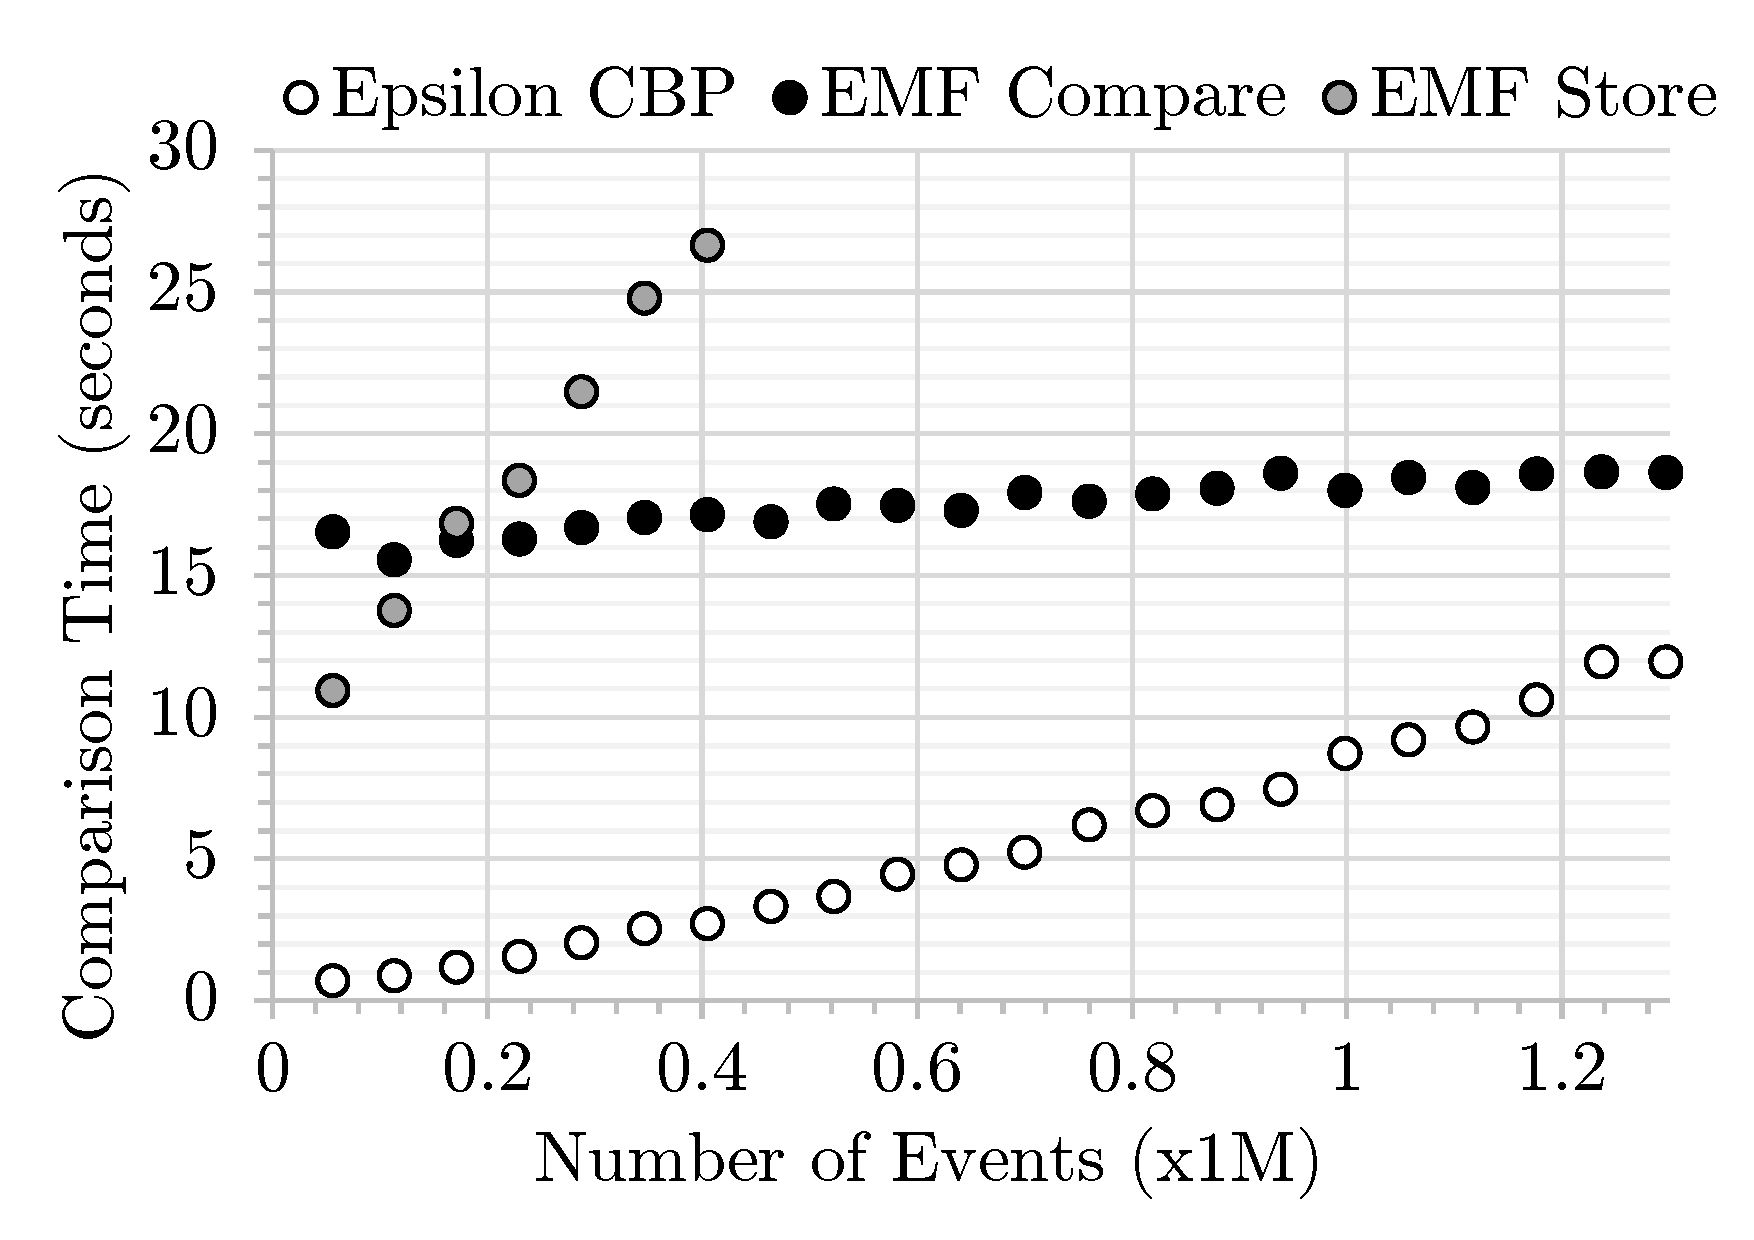
\includegraphics[width=\linewidth]{move-conflict-time-events}
    \caption{move-only}
    \label{fig:move-conflict-time-events}
  \end{subfigure}
  \hfill
  \begin{subfigure}[t]{0.495\linewidth}
    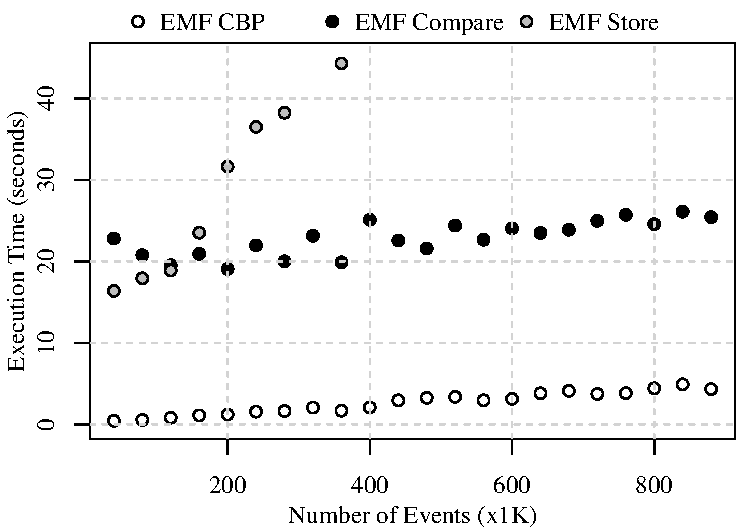
\includegraphics[width=\linewidth]{change-conflict-time-events}
    \caption{change-only}
    \label{fig:change-conflict-time-events}
  \end{subfigure}
  \caption{Conflict detection time for homogeneous operations.}
  \label{fig:homgeneous_operation_time_events}
\end{figure*}

\subsection{Homogenous Operations}
\label{sec:homogenous-operation_conflict}

\textbf{Detection Time}. Figure \ref{fig:homgeneous_operation_time_events} depicts the results of conflict detection time between Epsilon CBP, EMF Compare, and EMF Store in the context of homogenous operations. The results show that, in all types of homogenous operations, Epsilon CBP is the fastest on detecting conflicts compared to EMF Compare and EMF Store, while EMF Store has the worst performance. 

\textbf{Memory Footprint}. Figure \ref{fig:homgeneous_operation_memory_events} exhibits the memory footprint resulting from conflict detection in Epsilon CBP, EMF Compare, and EMF Store in the context of homogenous operations. The Figure displays that Epsilon CBP also outperforms EMF Compare and EMF Store in in terms of memory footprint. Epsilon CBP only performs worse than EMF Compare in delete-only operation, Figure \ref{fig:delete-conflict-memory-events} at a later stage when the number of events is over 0.22 millions.  

\begin{figure*}[ht]
  \centering
  \begin{subfigure}[t]{0.495\linewidth}
    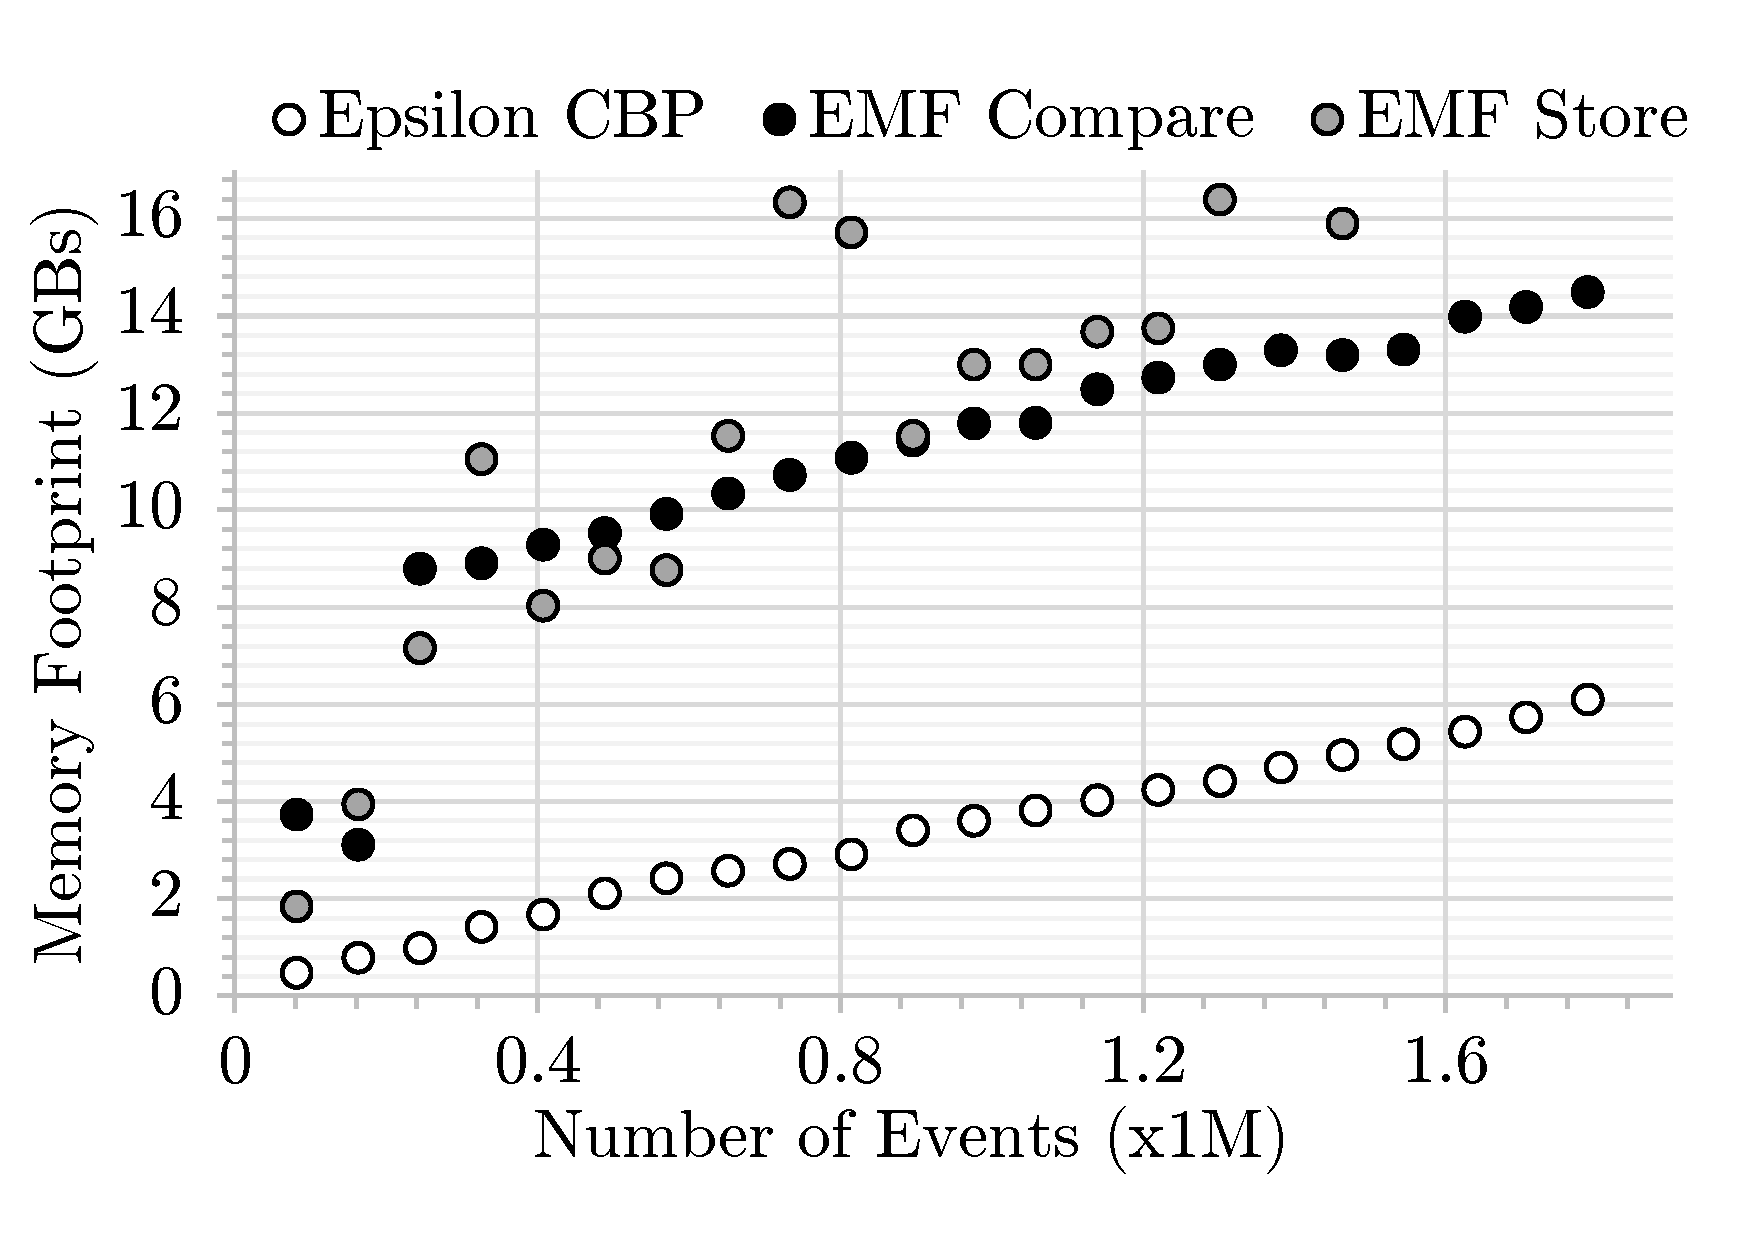
\includegraphics[width=\linewidth]{add-conflict-memory-events}
    \caption{add-only}
    \label{fig:add-conflict-memory-events}
  \end{subfigure}
  \hfill
  \begin{subfigure}[t]{0.495\linewidth}
    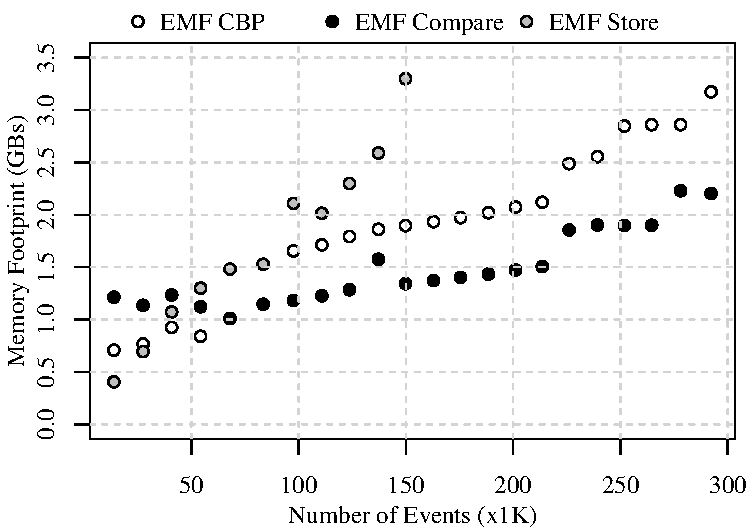
\includegraphics[width=\linewidth]{delete-conflict-memory-events}
    \caption{delete-only}
    \label{fig:delete-conflict-memory-events}
  \end{subfigure}
  \\
  \begin{subfigure}[t]{0.495\linewidth}
    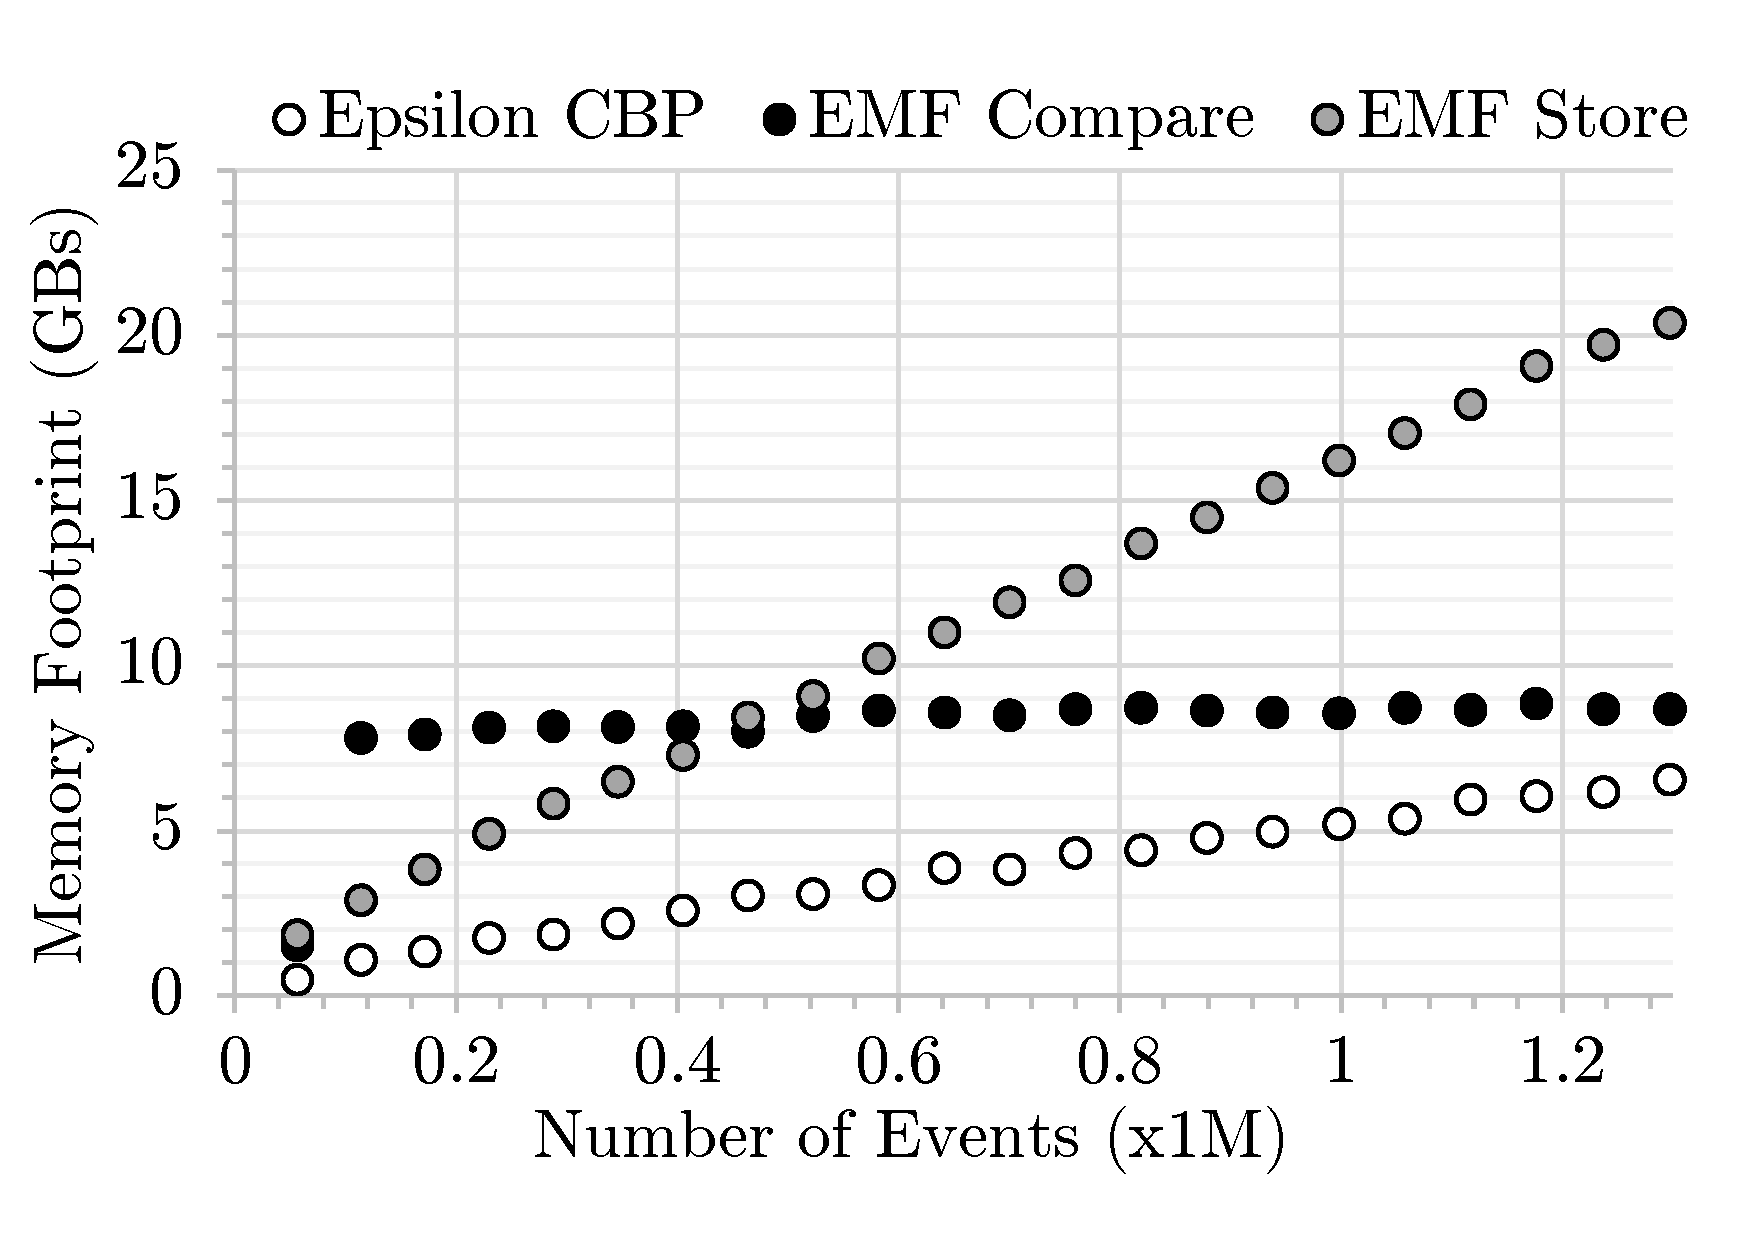
\includegraphics[width=\linewidth]{move-conflict-memory-events}
    \caption{move-only}
    \label{fig:move-conflict-memory-events}
  \end{subfigure}
  \hfill
  \begin{subfigure}[t]{0.495\linewidth}
    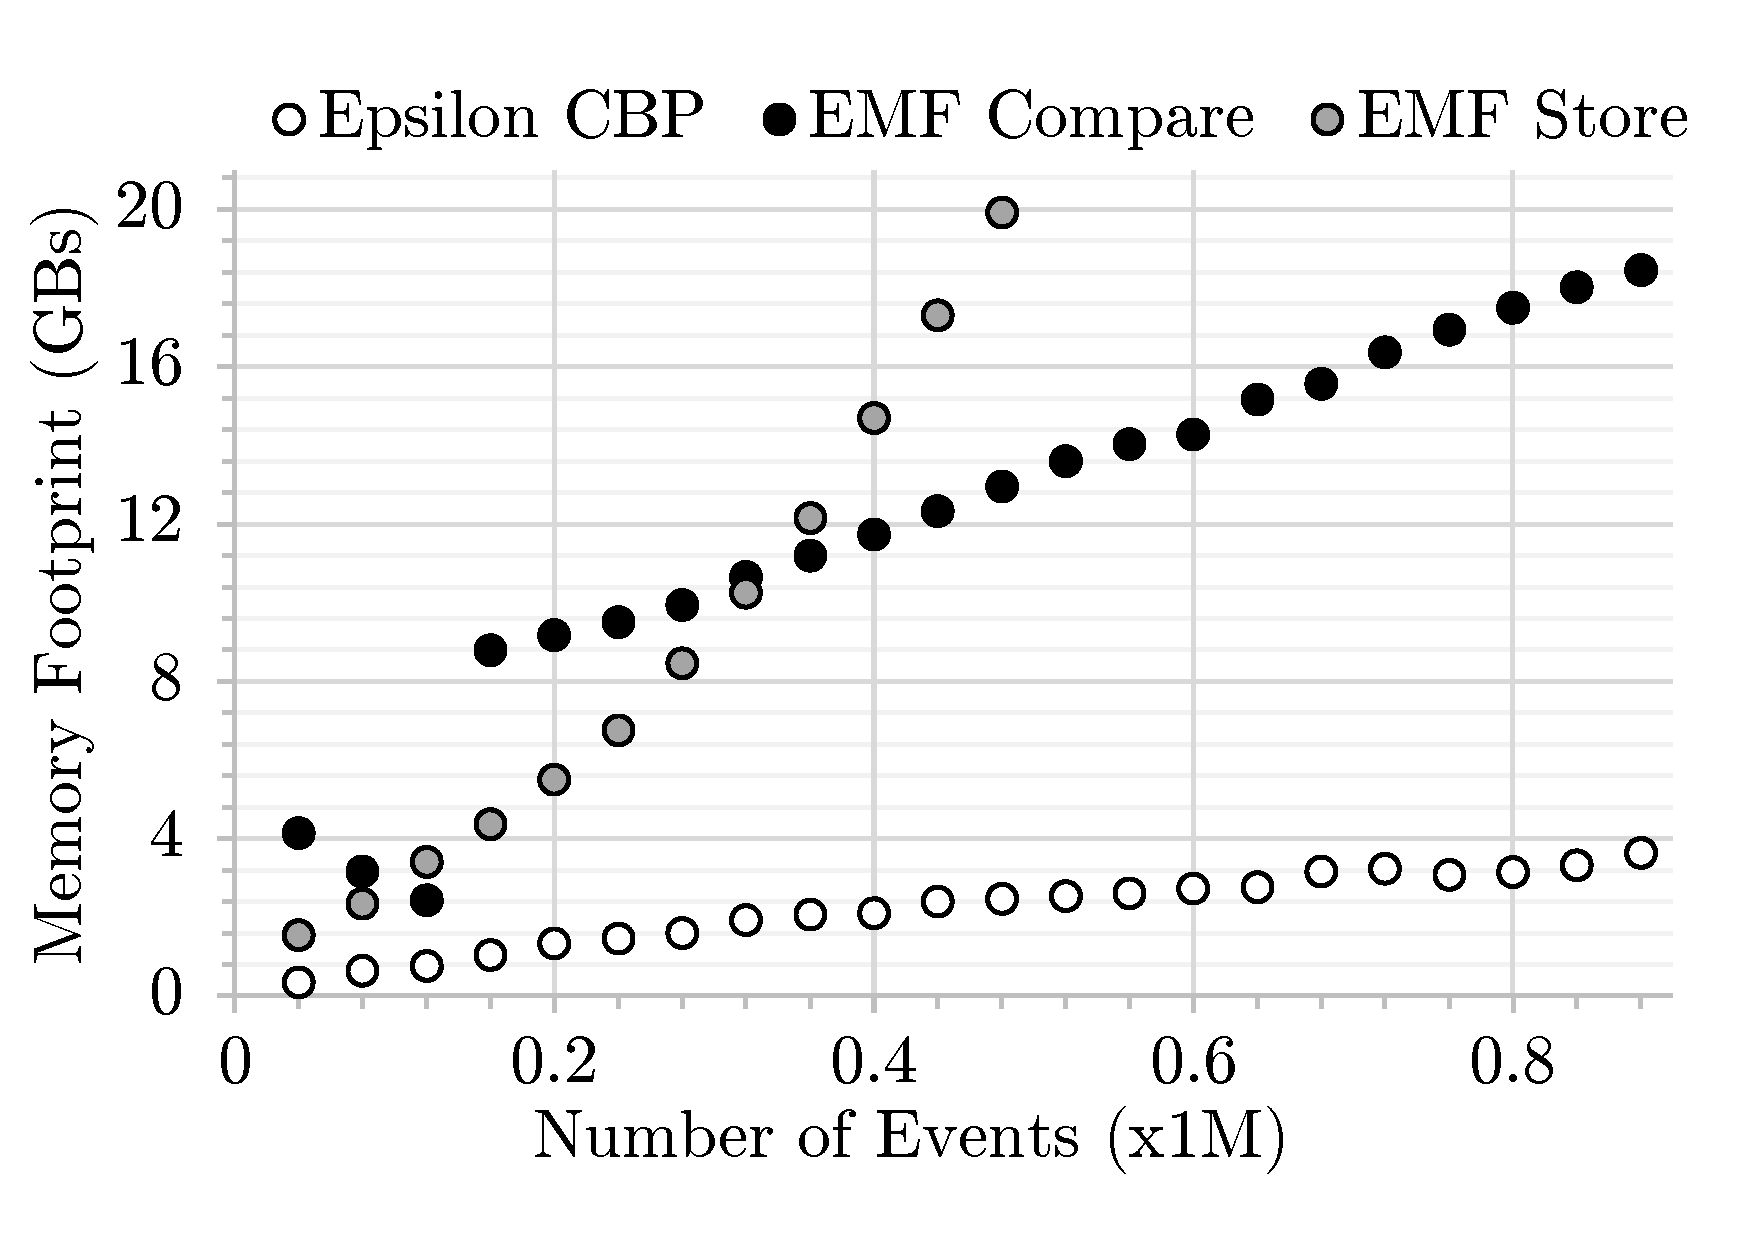
\includegraphics[width=\linewidth]{change-conflict-memory-events}
    \caption{change-only}
    \label{fig:change-conflict-memory-events}
  \end{subfigure}
  \caption{Conflict detection memory for homogeneous operations.}
  \label{fig:homgeneous_operation_memory_events}
\end{figure*}

In Figure \ref{fig:move-conflict-memory-events}, Epsilon CBP's memory footprint tends to increase faster than EMF Compare's memory footprint. This is possible since the change events of EMF Compare are actually optimal differences that derived from model differencing which in terms of number is less than real change events recorded in Epsilon CBP. 

\textbf{Conflict Count}. Figure \ref{fig:homgeneous_operation_count_events} displays the number of conflicts, both \textsf{REAL} and \textsf{PSEUDO}, detected by Epsilon CBP, EMF Compare, and EMF Store in the context of homogenous operations. In the add-only experiment as displayed in Figure \ref{fig:add-conflict-count-events}, three of them detect the same number of conflicts.

\begin{figure*}[ht]
  \centering
  \begin{subfigure}[t]{0.495\linewidth}
    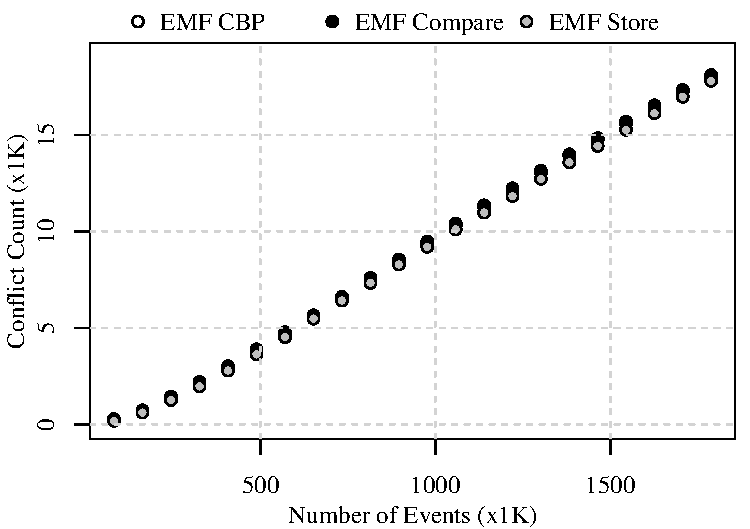
\includegraphics[width=\linewidth]{add-conflict-count-events}
    \caption{add-only}
    \label{fig:add-conflict-count-events}
  \end{subfigure}
  \hfill
  \begin{subfigure}[t]{0.495\linewidth}
    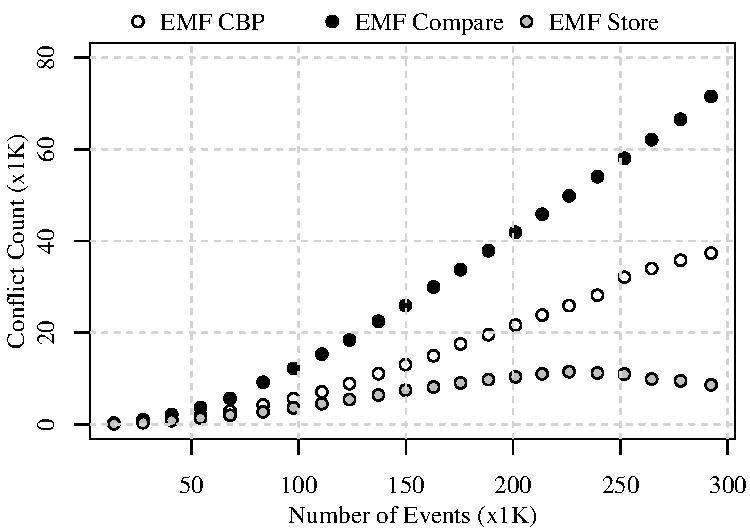
\includegraphics[width=\linewidth]{delete-conflict-count-events}
    \caption{delete-only}
    \label{fig:delete-conflict-count-events}
  \end{subfigure}
  \\
  \begin{subfigure}[t]{0.495\linewidth}
    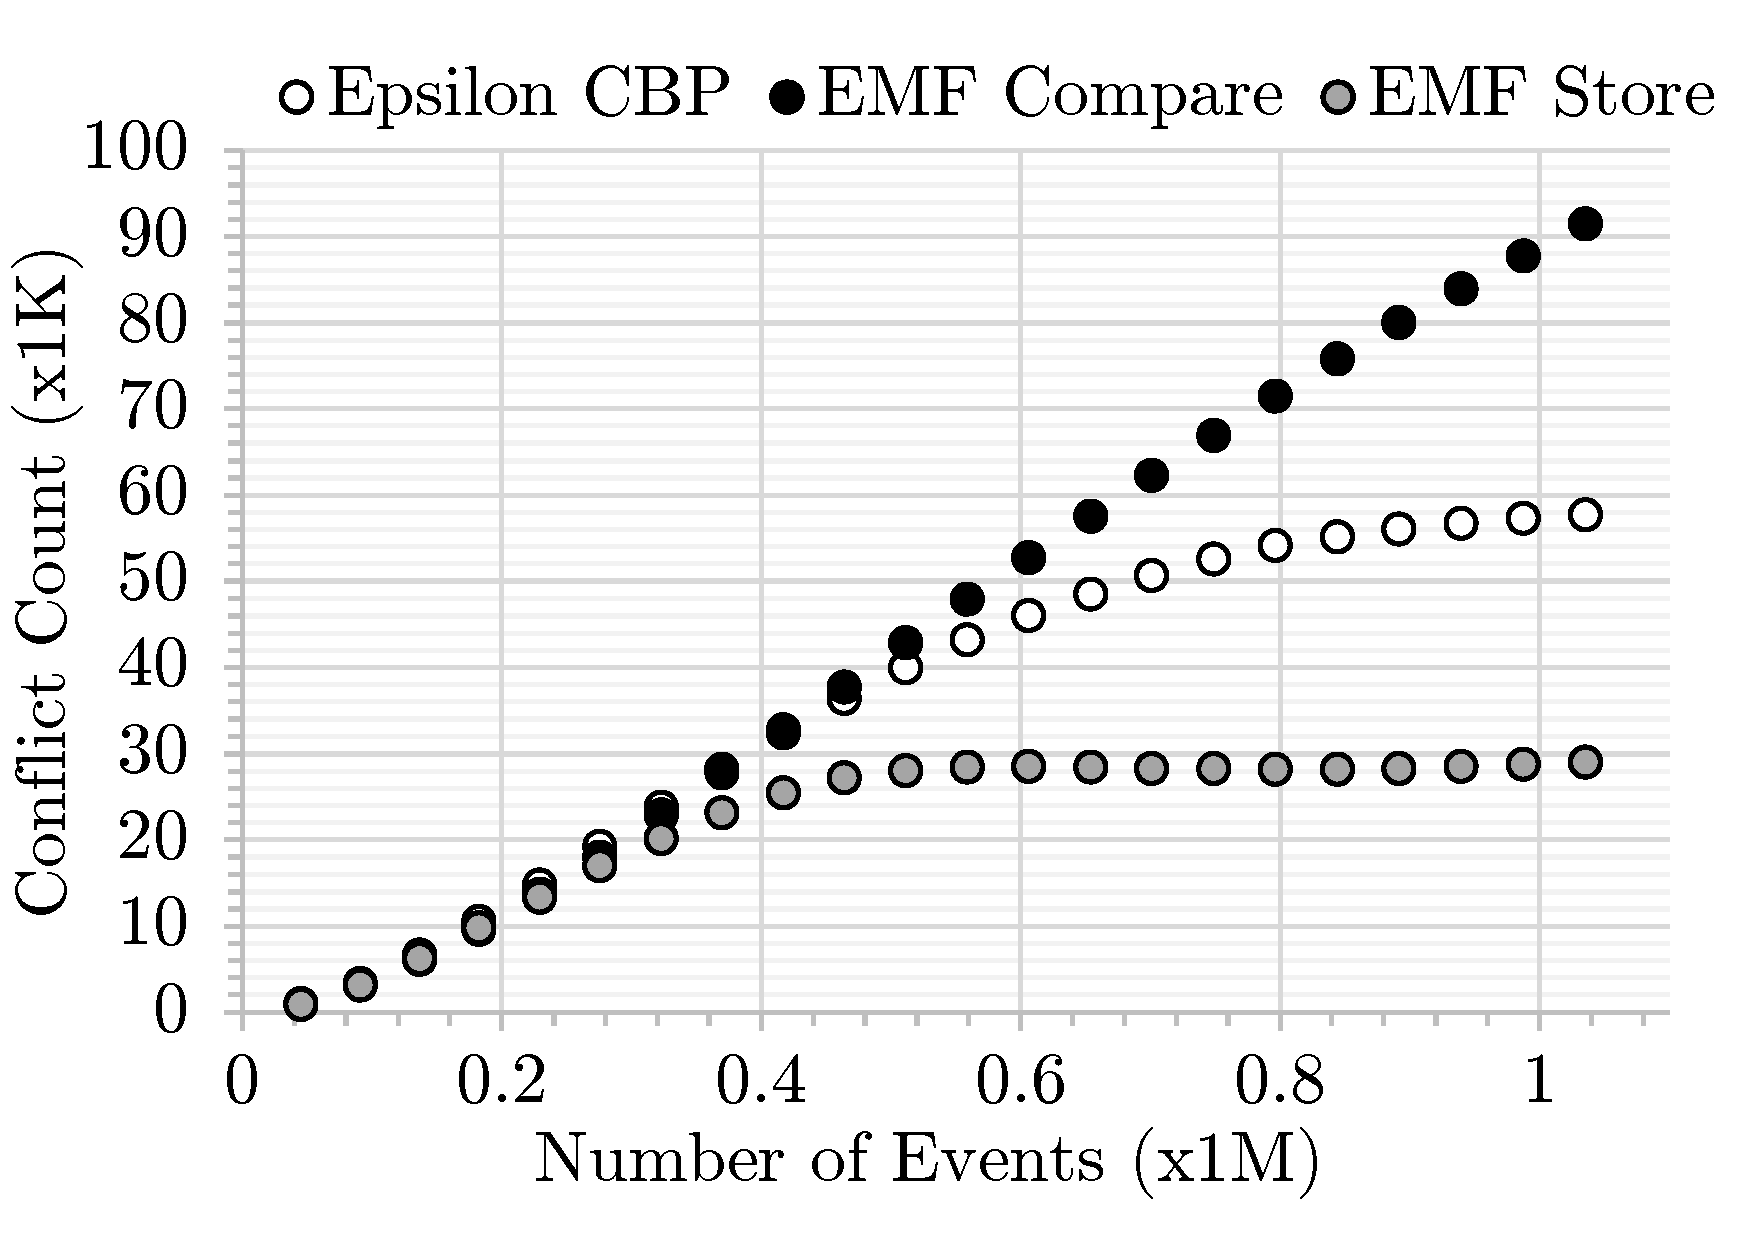
\includegraphics[width=\linewidth]{move-conflict-count-events}
    \caption{move-only}
    \label{fig:move-conflict-count-events}
  \end{subfigure}
  \hfill
  \begin{subfigure}[t]{0.495\linewidth}
    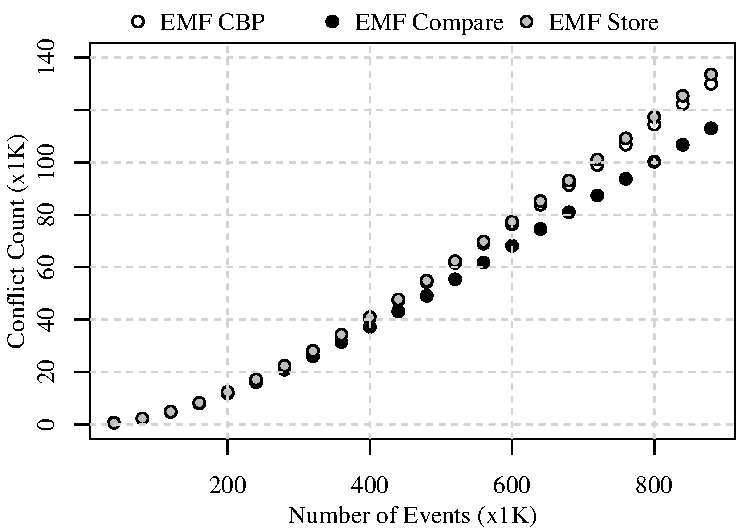
\includegraphics[width=\linewidth]{change-conflict-count-events}
    \caption{change-only}
    \label{fig:change-conflict-count-events}
  \end{subfigure}
  \caption{Conflict detection count for homogeneous operations.}
  \label{fig:homgeneous_operation_count_events}
\end{figure*}

Figure \ref{fig:change-conflict-count-events} shows the results of the change-only experiment. It can be noticed that the number of conflicts detected by EMF Compare is lower than Epsilon. This is due to EMF Compare that detects no change on an element or feature that has been modified but finally changed back to its original state. While in Epsilon CBP, this is counted as a change which is potential to raise a {PSEUDO} conflict as defined and showed in (\ref{eq:ecbp_pseudoconflict}) and Figure \ref{fig:statechart_04}. It can also be noticed that the number of conflicts detected by Epsilon CBP is slightly less than EMF Store detects. It is possible since EMF Store does not consider states in detecting conflicts thus two different change events that are applied to a same element or feature, even though they yield equivalent eventual states, are considered in conflict.

In the delete-only experiment as displayed in Figure \ref{fig:delete-conflict-count-events}, EMF Compare detects more conflicts than the others since it does not put conflicts that depends on other conflicts into one group, while EMF Store and Epsilon can automatically perform this grouping through composite events and the mapping of changes events to elements, features, and values that they affect. For example, the deletion of elements \textsf{cast} and \textsf{giant}, as showed in Table \ref{table:emfc_conflicts} are seperated into two conflicts, EC3 and EC4, while in EMF Store and Epsilon CBP group both deletion into one conflict as they are in in the same composite event \textsf{l2} (see conflict ES4 in Table \ref{table:conflicts_emfs}, conflict CB3 in Table \ref{table:conflicts_cbp}). Also, after deeper investigation, it is found that there is a bug in EMF Store that it cannot detect conflicts that involve deletion of elements in bidirectional features; error on reading element ids. Thus, it detects less conflicts than Epsilon CBP in delete-only experiment. 

Figure \ref{fig:move-conflict-count-events} shows the results of the move-only experiment. With the same reason to the results in the delete-only experiment -- conflicts are not grouped, EMF Compare detects more conflicts than EMF Store and Epsilon CBP. Specifically to EMF Store, it detects less conflicts than Epsilon CBP. After deeper investigation on the technical level, it is found that EMF Store cannot detect conflicts between left and right move events of an element, when they are preceded with other left and right move events of the same element. A conflict can only be detected if the left and right move events is the first events applied to the element.

\subsection{Conclusions}
\label{sec:conclusions_7}
Based on the findings in conflict detection evaluation, this study argues that the proposed change-based model conflict detection approach outperforms the conflict detection approaches in EMF Compare and EMF Store. Models that have been excessively modified and experience significant reduction on model size could impair the performance of the conflict detection as a great number of change records have to be read and loaded into memory. 

